\documentclass[twoside]{book}

% Packages required by doxygen
\usepackage{fixltx2e}
\usepackage{calc}
\usepackage{doxygen}
\usepackage[export]{adjustbox} % also loads graphicx
\usepackage{graphicx}
\usepackage[utf8]{inputenc}
\usepackage{makeidx}
\usepackage{multicol}
\usepackage{multirow}
\PassOptionsToPackage{warn}{textcomp}
\usepackage{textcomp}
\usepackage[nointegrals]{wasysym}
\usepackage[table]{xcolor}

% Font selection
\usepackage[T1]{fontenc}
\usepackage[scaled=.90]{helvet}
\usepackage{courier}
\usepackage{amssymb}
\usepackage{sectsty}
\renewcommand{\familydefault}{\sfdefault}
\allsectionsfont{%
  \fontseries{bc}\selectfont%
  \color{darkgray}%
}
\renewcommand{\DoxyLabelFont}{%
  \fontseries{bc}\selectfont%
  \color{darkgray}%
}
\newcommand{\+}{\discretionary{\mbox{\scriptsize$\hookleftarrow$}}{}{}}

% Page & text layout
\usepackage{geometry}
\geometry{%
  a4paper,%
  top=2.5cm,%
  bottom=2.5cm,%
  left=2.5cm,%
  right=2.5cm%
}
\tolerance=750
\hfuzz=15pt
\hbadness=750
\setlength{\emergencystretch}{15pt}
\setlength{\parindent}{0cm}
\setlength{\parskip}{3ex plus 2ex minus 2ex}
\makeatletter
\renewcommand{\paragraph}{%
  \@startsection{paragraph}{4}{0ex}{-1.0ex}{1.0ex}{%
    \normalfont\normalsize\bfseries\SS@parafont%
  }%
}
\renewcommand{\subparagraph}{%
  \@startsection{subparagraph}{5}{0ex}{-1.0ex}{1.0ex}{%
    \normalfont\normalsize\bfseries\SS@subparafont%
  }%
}
\makeatother

% Headers & footers
\usepackage{fancyhdr}
\pagestyle{fancyplain}
\fancyhead[LE]{\fancyplain{}{\bfseries\thepage}}
\fancyhead[CE]{\fancyplain{}{}}
\fancyhead[RE]{\fancyplain{}{\bfseries\leftmark}}
\fancyhead[LO]{\fancyplain{}{\bfseries\rightmark}}
\fancyhead[CO]{\fancyplain{}{}}
\fancyhead[RO]{\fancyplain{}{\bfseries\thepage}}
\fancyfoot[LE]{\fancyplain{}{}}
\fancyfoot[CE]{\fancyplain{}{}}
\fancyfoot[RE]{\fancyplain{}{\bfseries\scriptsize Generated by Doxygen }}
\fancyfoot[LO]{\fancyplain{}{\bfseries\scriptsize Generated by Doxygen }}
\fancyfoot[CO]{\fancyplain{}{}}
\fancyfoot[RO]{\fancyplain{}{}}
\renewcommand{\footrulewidth}{0.4pt}
\renewcommand{\chaptermark}[1]{%
  \markboth{#1}{}%
}
\renewcommand{\sectionmark}[1]{%
  \markright{\thesection\ #1}%
}

% Indices & bibliography
\usepackage{natbib}
\usepackage[titles]{tocloft}
\setcounter{tocdepth}{3}
\setcounter{secnumdepth}{5}
\makeindex

% Hyperlinks (required, but should be loaded last)
\usepackage{ifpdf}
\ifpdf
  \usepackage[pdftex,pagebackref=true]{hyperref}
\else
  \usepackage[ps2pdf,pagebackref=true]{hyperref}
\fi
\hypersetup{%
  colorlinks=true,%
  linkcolor=blue,%
  citecolor=blue,%
  unicode%
}

% Custom commands
\newcommand{\clearemptydoublepage}{%
  \newpage{\pagestyle{empty}\cleardoublepage}%
}

\usepackage{caption}
\captionsetup{labelsep=space,justification=centering,font={bf},singlelinecheck=off,skip=4pt,position=top}

%===== C O N T E N T S =====

\begin{document}

% Titlepage & ToC
\hypersetup{pageanchor=false,
             bookmarksnumbered=true,
             pdfencoding=unicode
            }
\pagenumbering{alph}
\begin{titlepage}
\vspace*{7cm}
\begin{center}%
{\Large My Project }\\
\vspace*{1cm}
{\large Generated by Doxygen 1.8.14}\\
\end{center}
\end{titlepage}
\clearemptydoublepage
\pagenumbering{roman}
\tableofcontents
\clearemptydoublepage
\pagenumbering{arabic}
\hypersetup{pageanchor=true}

%--- Begin generated contents ---
\chapter{Hierarchical Index}
\section{Class Hierarchy}
This inheritance list is sorted roughly, but not completely, alphabetically\+:\begin{DoxyCompactList}
\item \contentsline{section}{Area}{\pageref{class_area}}{}
\begin{DoxyCompactList}
\item \contentsline{section}{Rect\+Area}{\pageref{class_rect_area}}{}
\begin{DoxyCompactList}
\item \contentsline{section}{Area11}{\pageref{class_area11}}{}
\item \contentsline{section}{Area12}{\pageref{class_area12}}{}
\item \contentsline{section}{Area13}{\pageref{class_area13}}{}
\item \contentsline{section}{Area21}{\pageref{class_area21}}{}
\item \contentsline{section}{Area22}{\pageref{class_area22}}{}
\item \contentsline{section}{Area23}{\pageref{class_area23}}{}
\item \contentsline{section}{Area31}{\pageref{class_area31}}{}
\item \contentsline{section}{Area32}{\pageref{class_area32}}{}
\item \contentsline{section}{Area33}{\pageref{class_area33}}{}
\end{DoxyCompactList}
\end{DoxyCompactList}
\item \contentsline{section}{Function}{\pageref{class_function}}{}
\begin{DoxyCompactList}
\item \contentsline{section}{function1}{\pageref{classfunction1}}{}
\item \contentsline{section}{function2}{\pageref{classfunction2}}{}
\item \contentsline{section}{function3}{\pageref{classfunction3}}{}
\item \contentsline{section}{function4}{\pageref{classfunction4}}{}
\item \contentsline{section}{function5}{\pageref{classfunction5}}{}
\end{DoxyCompactList}
\item \contentsline{section}{Optimization\+Method}{\pageref{class_optimization_method}}{}
\begin{DoxyCompactList}
\item \contentsline{section}{Fletcher\+Reeves\+CG}{\pageref{class_fletcher_reeves_c_g}}{}
\item \contentsline{section}{Stochastic}{\pageref{class_stochastic}}{}
\end{DoxyCompactList}
\item \contentsline{section}{Stop\+Criterion}{\pageref{class_stop_criterion}}{}
\begin{DoxyCompactList}
\item \contentsline{section}{coord}{\pageref{classcoord}}{}
\item \contentsline{section}{last\+\_\+improv}{\pageref{classlast__improv}}{}
\item \contentsline{section}{n\+\_\+iter}{\pageref{classn__iter}}{}
\item \contentsline{section}{nabla}{\pageref{classnabla}}{}
\item \contentsline{section}{value}{\pageref{classvalue}}{}
\end{DoxyCompactList}
\end{DoxyCompactList}

\chapter{Class Index}
\section{Class List}
Here are the classes, structs, unions and interfaces with brief descriptions\+:\begin{DoxyCompactList}
\item\contentsline{section}{\mbox{\hyperlink{class_area}{Area}} }{\pageref{class_area}}{}
\item\contentsline{section}{\mbox{\hyperlink{class_area11}{Area11}} }{\pageref{class_area11}}{}
\item\contentsline{section}{\mbox{\hyperlink{class_area12}{Area12}} }{\pageref{class_area12}}{}
\item\contentsline{section}{\mbox{\hyperlink{class_area13}{Area13}} }{\pageref{class_area13}}{}
\item\contentsline{section}{\mbox{\hyperlink{class_area21}{Area21}} }{\pageref{class_area21}}{}
\item\contentsline{section}{\mbox{\hyperlink{class_area22}{Area22}} }{\pageref{class_area22}}{}
\item\contentsline{section}{\mbox{\hyperlink{class_area23}{Area23}} }{\pageref{class_area23}}{}
\item\contentsline{section}{\mbox{\hyperlink{class_area31}{Area31}} }{\pageref{class_area31}}{}
\item\contentsline{section}{\mbox{\hyperlink{class_area32}{Area32}} }{\pageref{class_area32}}{}
\item\contentsline{section}{\mbox{\hyperlink{class_area33}{Area33}} }{\pageref{class_area33}}{}
\item\contentsline{section}{\mbox{\hyperlink{classcoord}{coord}} }{\pageref{classcoord}}{}
\item\contentsline{section}{\mbox{\hyperlink{class_fletcher_reeves_c_g}{Fletcher\+Reeves\+CG}} }{\pageref{class_fletcher_reeves_c_g}}{}
\item\contentsline{section}{\mbox{\hyperlink{class_function}{Function}} }{\pageref{class_function}}{}
\item\contentsline{section}{\mbox{\hyperlink{classfunction1}{function1}} }{\pageref{classfunction1}}{}
\item\contentsline{section}{\mbox{\hyperlink{classfunction2}{function2}} }{\pageref{classfunction2}}{}
\item\contentsline{section}{\mbox{\hyperlink{classfunction3}{function3}} }{\pageref{classfunction3}}{}
\item\contentsline{section}{\mbox{\hyperlink{classfunction4}{function4}} }{\pageref{classfunction4}}{}
\item\contentsline{section}{\mbox{\hyperlink{classfunction5}{function5}} }{\pageref{classfunction5}}{}
\item\contentsline{section}{\mbox{\hyperlink{classlast__improv}{last\+\_\+improv}} }{\pageref{classlast__improv}}{}
\item\contentsline{section}{\mbox{\hyperlink{classn__iter}{n\+\_\+iter}} }{\pageref{classn__iter}}{}
\item\contentsline{section}{\mbox{\hyperlink{classnabla}{nabla}} }{\pageref{classnabla}}{}
\item\contentsline{section}{\mbox{\hyperlink{class_optimization_method}{Optimization\+Method}} }{\pageref{class_optimization_method}}{}
\item\contentsline{section}{\mbox{\hyperlink{class_rect_area}{Rect\+Area}} }{\pageref{class_rect_area}}{}
\item\contentsline{section}{\mbox{\hyperlink{class_stochastic}{Stochastic}} }{\pageref{class_stochastic}}{}
\item\contentsline{section}{\mbox{\hyperlink{class_stop_criterion}{Stop\+Criterion}} }{\pageref{class_stop_criterion}}{}
\item\contentsline{section}{\mbox{\hyperlink{classvalue}{value}} }{\pageref{classvalue}}{}
\end{DoxyCompactList}

\chapter{Class Documentation}
\hypertarget{class_area}{}\section{Area Class Reference}
\label{class_area}\index{Area@{Area}}


{\ttfamily \#include $<$Area.\+h$>$}

Inheritance diagram for Area\+:\begin{figure}[H]
\begin{center}
\leavevmode
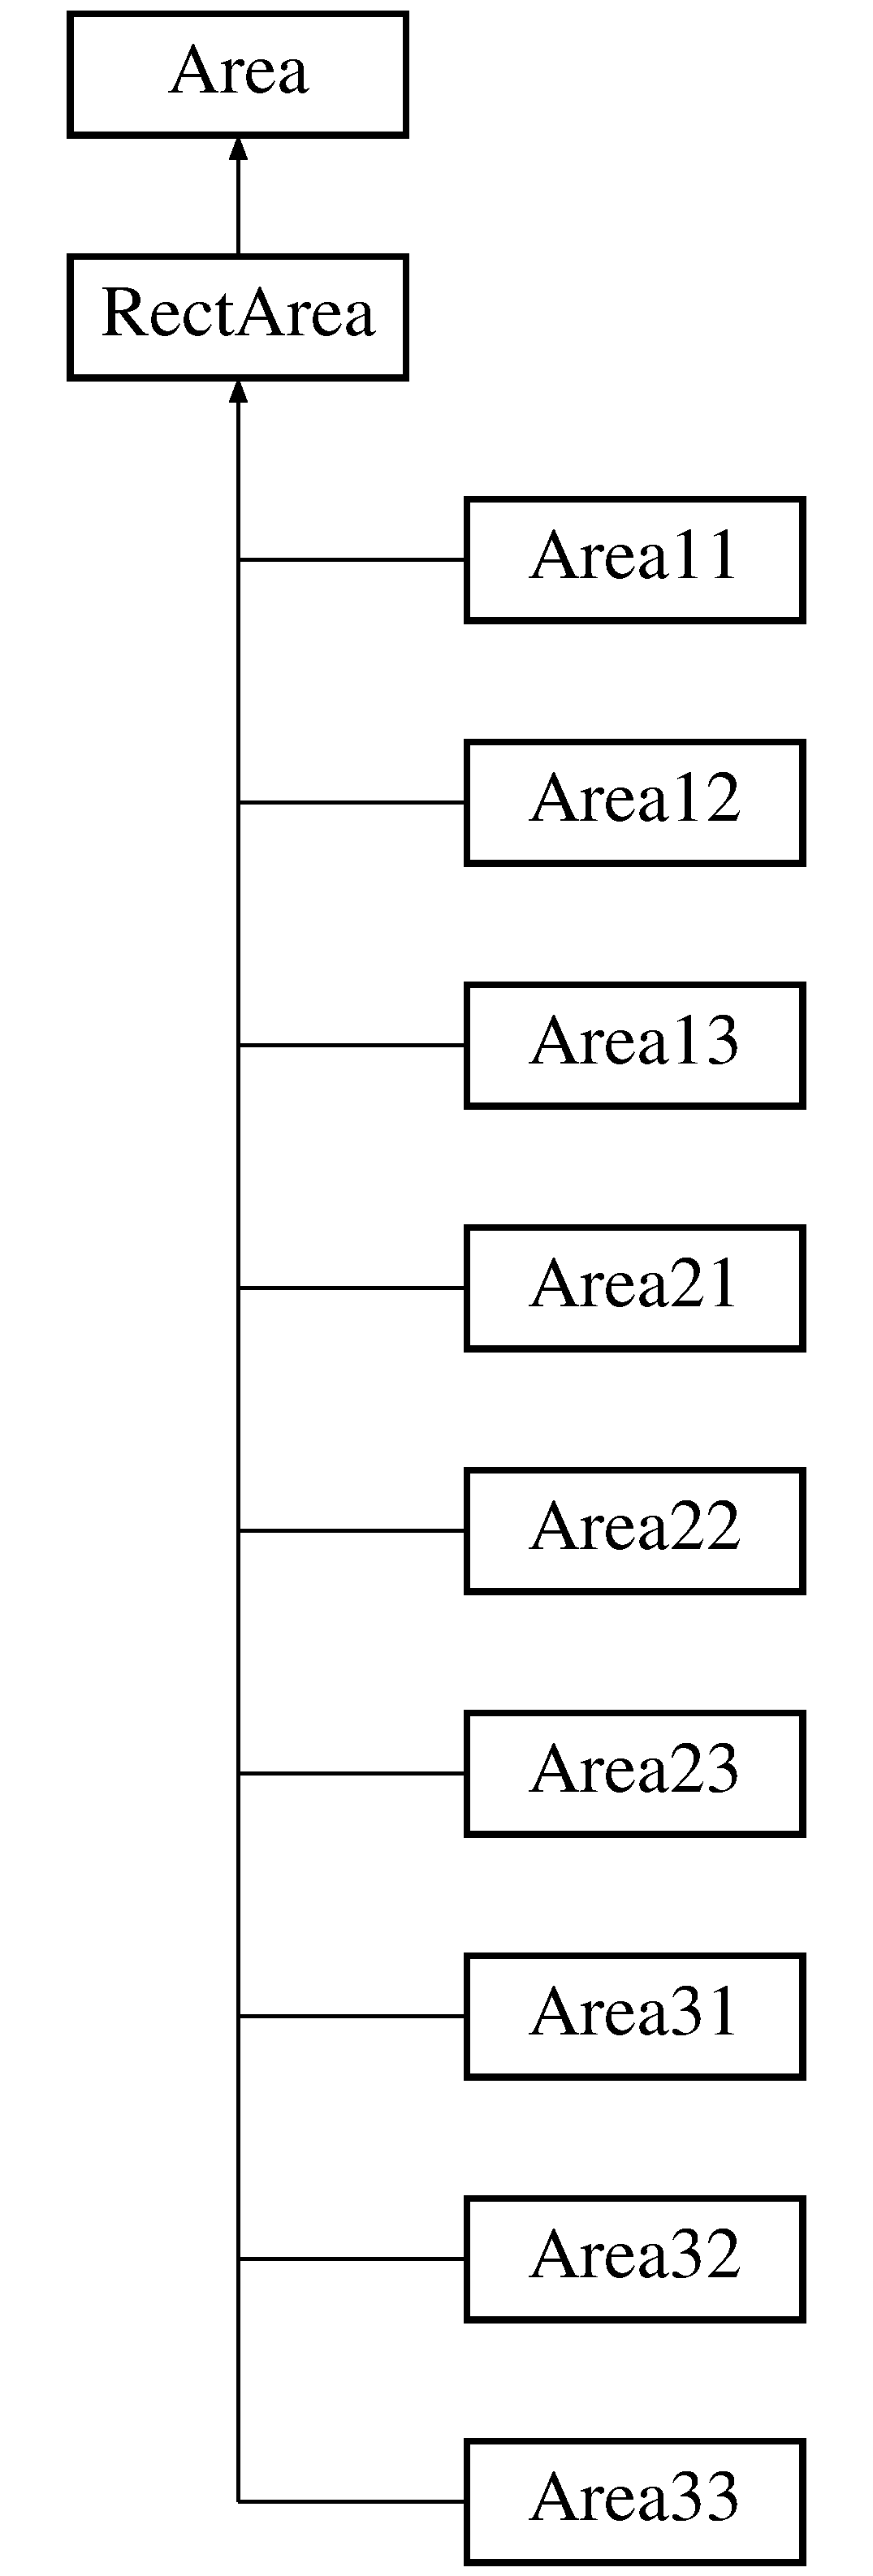
\includegraphics[height=11.000000cm]{class_area}
\end{center}
\end{figure}
\subsection*{Public Member Functions}
\begin{DoxyCompactItemize}
\item 
\mbox{\Hypertarget{class_area_ace56b94df20ea28011b3a9cd95dc1822}\label{class_area_ace56b94df20ea28011b3a9cd95dc1822}} 
{\bfseries Area} (int n, std\+::vector$<$ double $>$ dot)
\item 
bool \mbox{\hyperlink{class_area_a51d5a60d36a0fd4c45eb374eea1bc976}{Is\+In\+Area}} (std\+::vector$<$ double $>$ x, double eps)
\item 
\mbox{\Hypertarget{class_area_a0981bb64103aa1fada5c4eb015d16728}\label{class_area_a0981bb64103aa1fada5c4eb015d16728}} 
int {\bfseries Get\+Dimension} ()
\item 
\mbox{\Hypertarget{class_area_a976037f5d9dace960388d0bfcfaf1d01}\label{class_area_a976037f5d9dace960388d0bfcfaf1d01}} 
std\+::vector$<$ double $>$ {\bfseries Get\+Border} ()
\end{DoxyCompactItemize}
\subsection*{Protected Attributes}
\begin{DoxyCompactItemize}
\item 
\mbox{\Hypertarget{class_area_a4ec26baccd65af0189a9c8c25ab86ec3}\label{class_area_a4ec26baccd65af0189a9c8c25ab86ec3}} 
int \mbox{\hyperlink{class_area_a4ec26baccd65af0189a9c8c25ab86ec3}{dimension}}
\begin{DoxyCompactList}\small\item\em Размерность области \end{DoxyCompactList}\item 
\mbox{\Hypertarget{class_area_abfef011384225390a16165cd89f5d69d}\label{class_area_abfef011384225390a16165cd89f5d69d}} 
std\+::vector$<$ double $>$ \mbox{\hyperlink{class_area_abfef011384225390a16165cd89f5d69d}{border}}
\begin{DoxyCompactList}\small\item\em Граница области \end{DoxyCompactList}\end{DoxyCompactItemize}


\subsection{Detailed Description}
В данном классе определяются возможные заданные области, предоставляемые пользователю на выбор. 

\subsection{Member Function Documentation}
\mbox{\Hypertarget{class_area_a51d5a60d36a0fd4c45eb374eea1bc976}\label{class_area_a51d5a60d36a0fd4c45eb374eea1bc976}} 
\index{Area@{Area}!Is\+In\+Area@{Is\+In\+Area}}
\index{Is\+In\+Area@{Is\+In\+Area}!Area@{Area}}
\subsubsection{\texorpdfstring{Is\+In\+Area()}{IsInArea()}}
{\footnotesize\ttfamily bool Area\+::\+Is\+In\+Area (\begin{DoxyParamCaption}\item[{std\+::vector$<$ double $>$}]{x,  }\item[{double}]{eps }\end{DoxyParamCaption})}

Проверяет, находится ли переданная точка в текущей области с заданной погрешностью. 
\begin{DoxyParams}{Parameters}
{\em x} & Проверяемая точка \\
\hline
{\em eps} & Заданная погрешность \\
\hline
\end{DoxyParams}
\begin{DoxyReturn}{Returns}
1, если точка внутри области; 0, иначе 
\end{DoxyReturn}


The documentation for this class was generated from the following files\+:\begin{DoxyCompactItemize}
\item 
Area.\+h\item 
Area.\+cpp\end{DoxyCompactItemize}

\hypertarget{class_area11}{}\section{Area11 Class Reference}
\label{class_area11}\index{Area11@{Area11}}
Inheritance diagram for Area11\+:\begin{figure}[H]
\begin{center}
\leavevmode
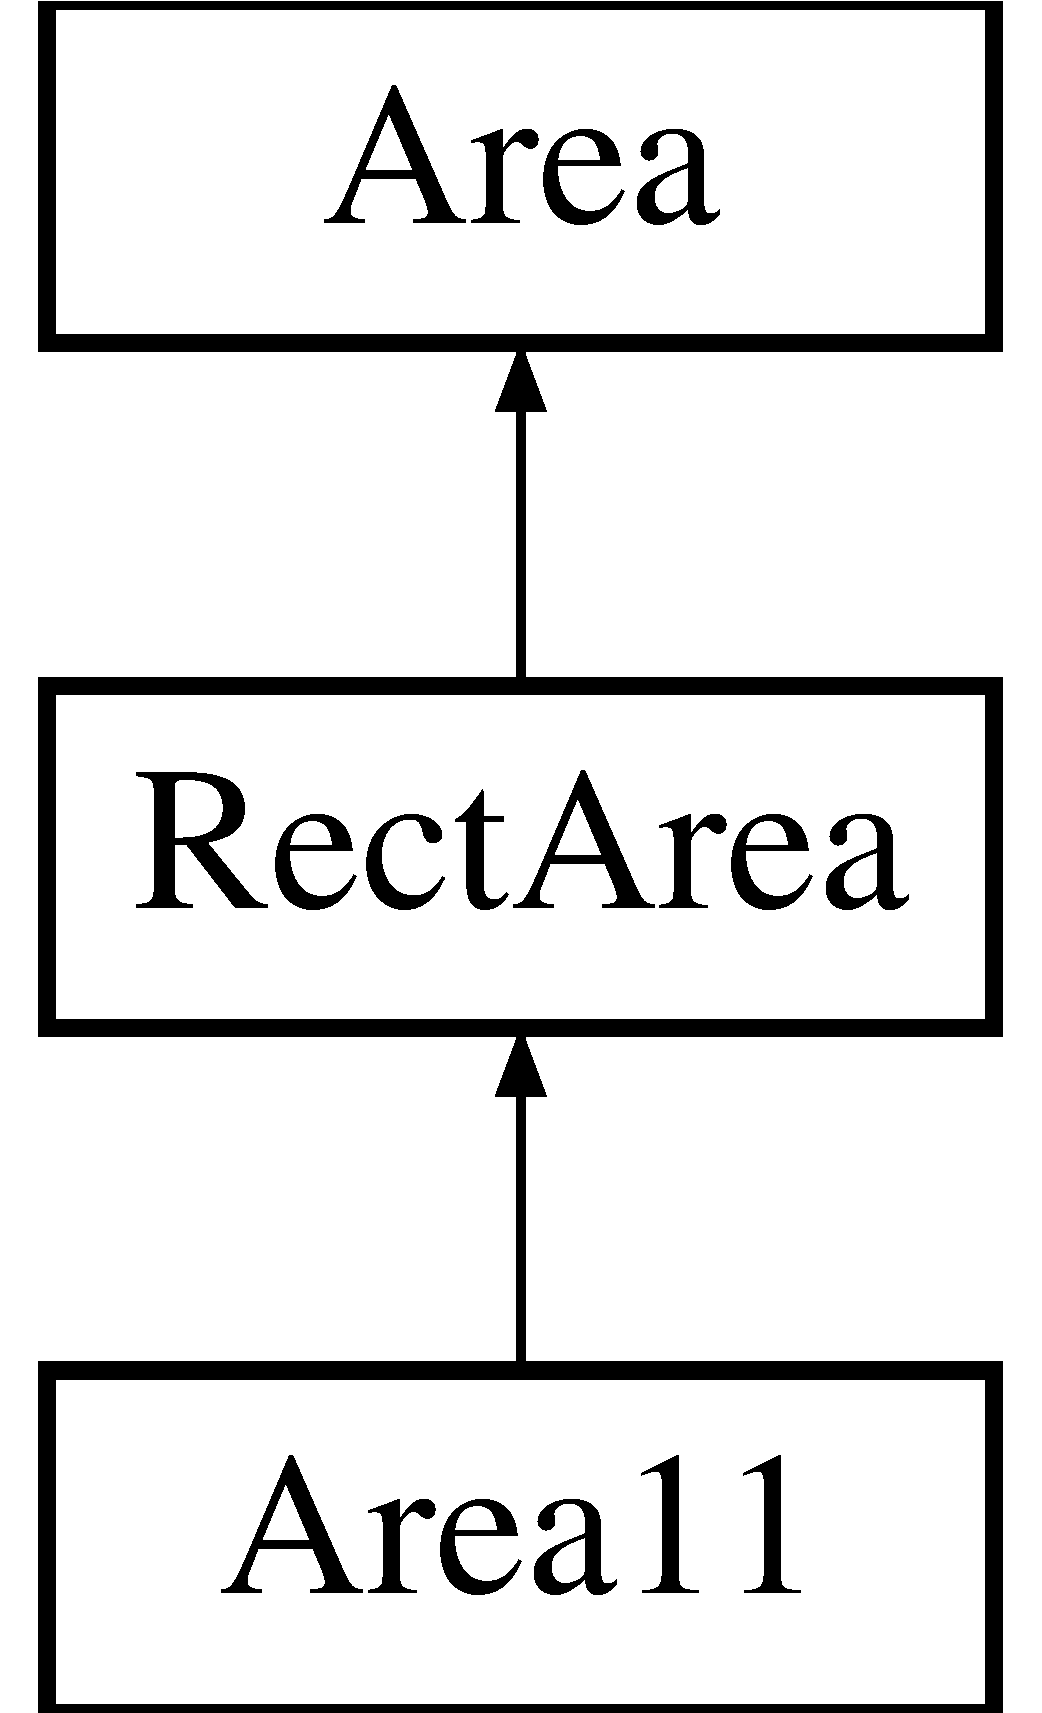
\includegraphics[height=3.000000cm]{class_area11}
\end{center}
\end{figure}
\subsection*{Public Member Functions}
\begin{DoxyCompactItemize}
\item 
\mbox{\Hypertarget{class_area11_aac2e4a6490509ad45aadf710ee10e91e}\label{class_area11_aac2e4a6490509ad45aadf710ee10e91e}} 
{\bfseries Area11} (int n=2, std\+::vector$<$ double $>$ dot=\{ 0, 3, 0, 3 \})
\end{DoxyCompactItemize}
\subsection*{Additional Inherited Members}


The documentation for this class was generated from the following file\+:\begin{DoxyCompactItemize}
\item 
Area.\+h\end{DoxyCompactItemize}

\hypertarget{class_area12}{}\section{Area12 Class Reference}
\label{class_area12}\index{Area12@{Area12}}
Inheritance diagram for Area12\+:\begin{figure}[H]
\begin{center}
\leavevmode
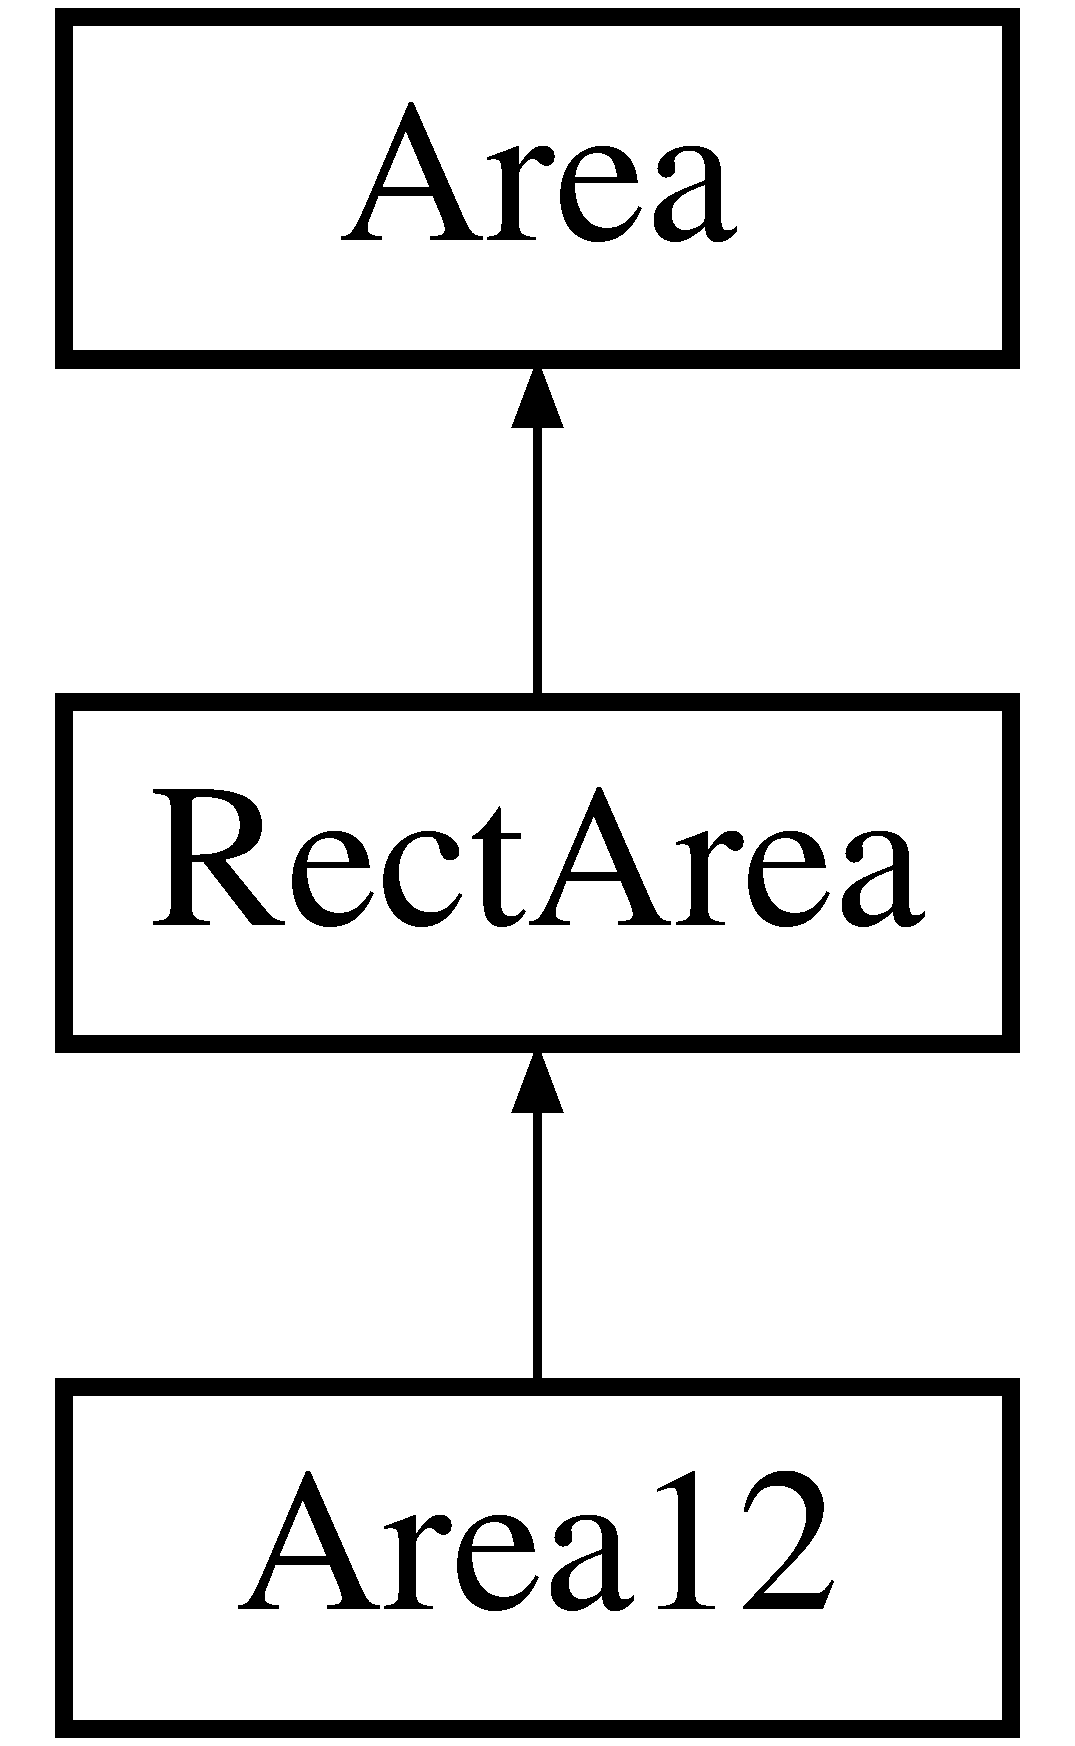
\includegraphics[height=3.000000cm]{class_area12}
\end{center}
\end{figure}
\subsection*{Public Member Functions}
\begin{DoxyCompactItemize}
\item 
\mbox{\Hypertarget{class_area12_aa1606d3d43a29ab16c47c642d356c5df}\label{class_area12_aa1606d3d43a29ab16c47c642d356c5df}} 
{\bfseries Area12} (int n=2, std\+::vector$<$ double $>$ dot=\{ 2, 5, 2, 5 \})
\end{DoxyCompactItemize}
\subsection*{Additional Inherited Members}


The documentation for this class was generated from the following file\+:\begin{DoxyCompactItemize}
\item 
Area.\+h\end{DoxyCompactItemize}

\hypertarget{class_area13}{}\section{Area13 Class Reference}
\label{class_area13}\index{Area13@{Area13}}
Inheritance diagram for Area13\+:\begin{figure}[H]
\begin{center}
\leavevmode
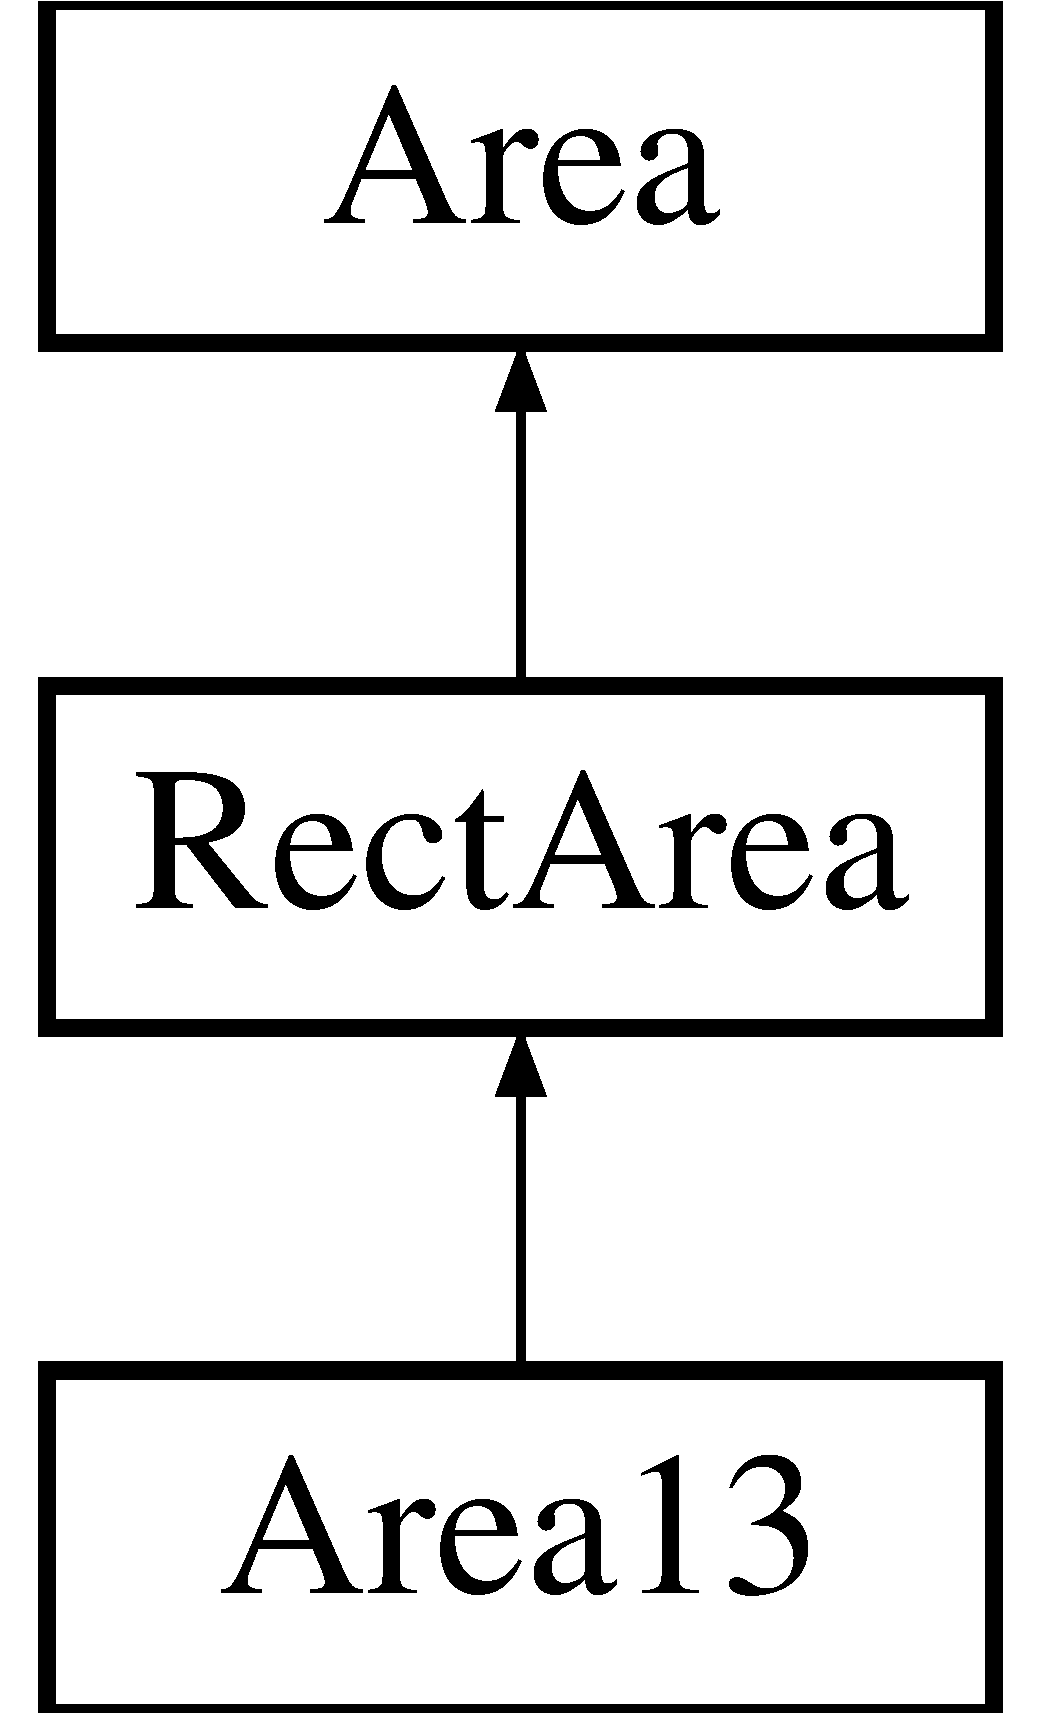
\includegraphics[height=3.000000cm]{class_area13}
\end{center}
\end{figure}
\subsection*{Public Member Functions}
\begin{DoxyCompactItemize}
\item 
\mbox{\Hypertarget{class_area13_ac4fc316009b697bb551bd816078564c9}\label{class_area13_ac4fc316009b697bb551bd816078564c9}} 
{\bfseries Area13} (int n=2, std\+::vector$<$ double $>$ dot=\{ -\/5, 5, -\/5, 5 \})
\end{DoxyCompactItemize}
\subsection*{Additional Inherited Members}


The documentation for this class was generated from the following file\+:\begin{DoxyCompactItemize}
\item 
Area.\+h\end{DoxyCompactItemize}

\hypertarget{class_area21}{}\section{Area21 Class Reference}
\label{class_area21}\index{Area21@{Area21}}
Inheritance diagram for Area21\+:\begin{figure}[H]
\begin{center}
\leavevmode
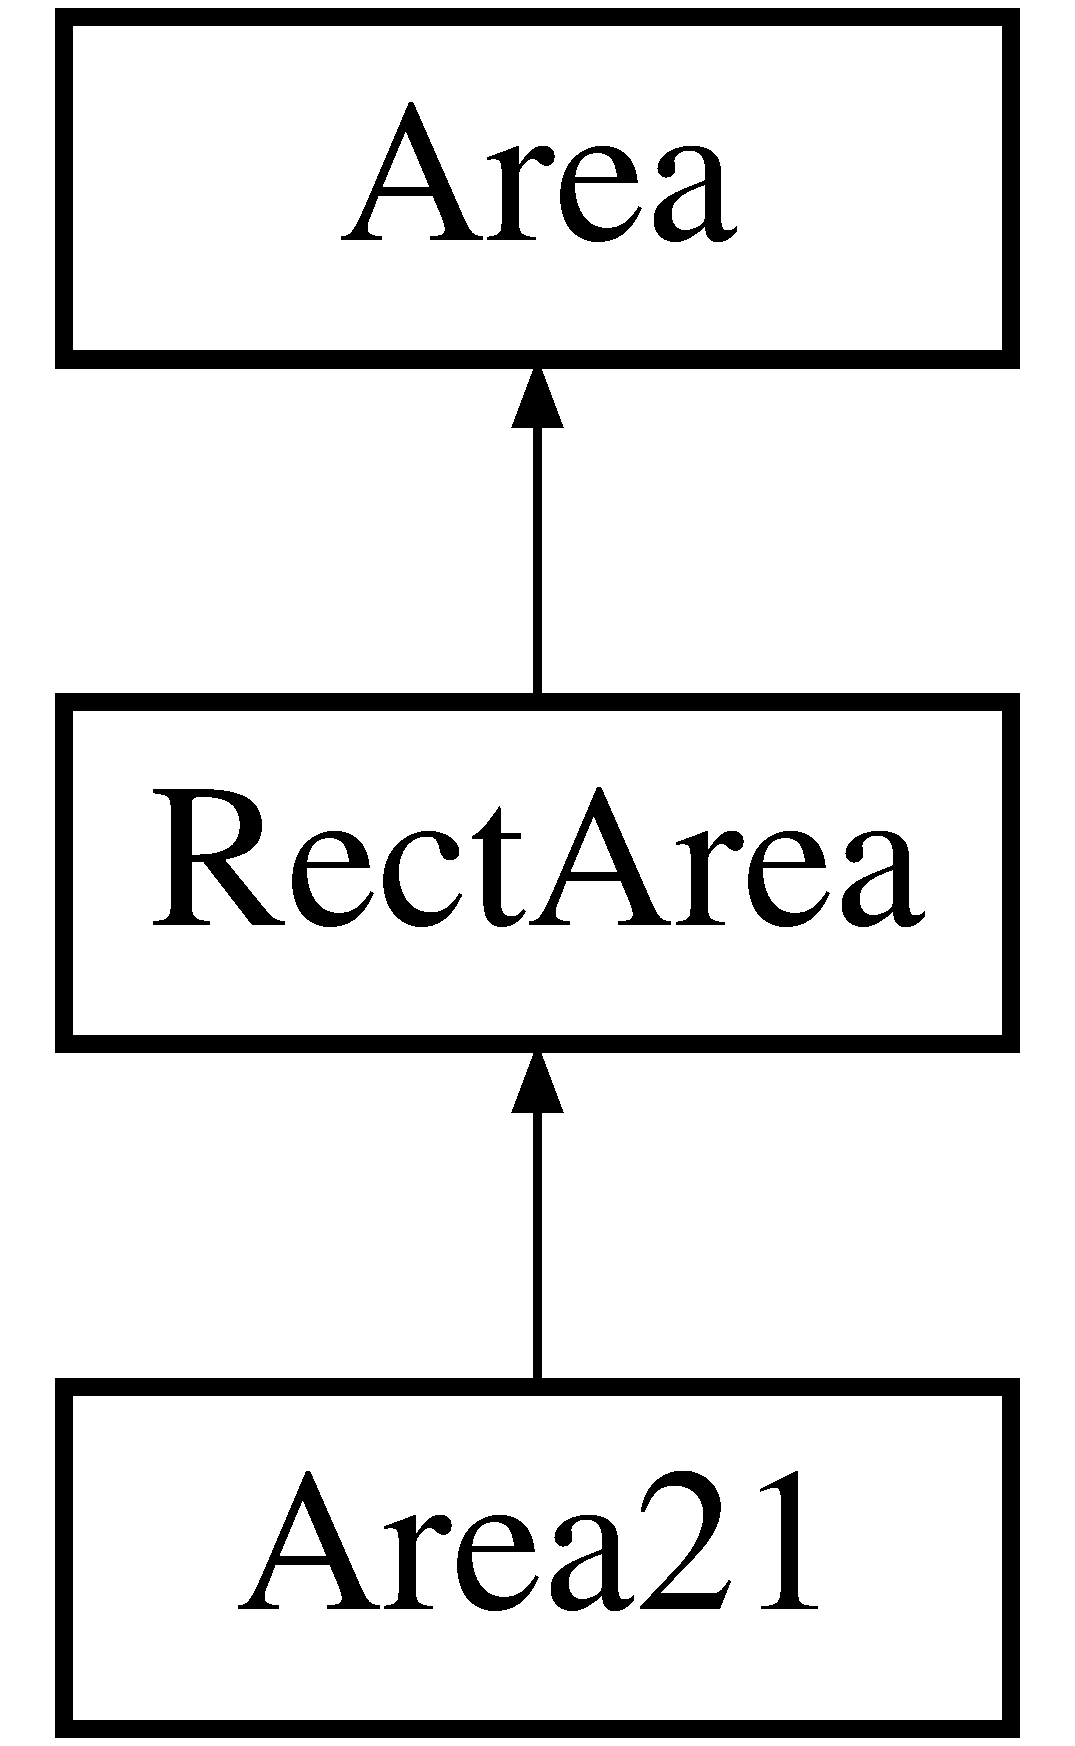
\includegraphics[height=3.000000cm]{class_area21}
\end{center}
\end{figure}
\subsection*{Public Member Functions}
\begin{DoxyCompactItemize}
\item 
\mbox{\Hypertarget{class_area21_ad83b437747cc5b94620fedb938158d5e}\label{class_area21_ad83b437747cc5b94620fedb938158d5e}} 
{\bfseries Area21} (int n=3, std\+::vector$<$ double $>$ dot=\{ 0, 3, 0, 3, 0, 3 \})
\end{DoxyCompactItemize}
\subsection*{Additional Inherited Members}


The documentation for this class was generated from the following file\+:\begin{DoxyCompactItemize}
\item 
Area.\+h\end{DoxyCompactItemize}

\hypertarget{class_area22}{}\section{Area22 Class Reference}
\label{class_area22}\index{Area22@{Area22}}
Inheritance diagram for Area22\+:\begin{figure}[H]
\begin{center}
\leavevmode
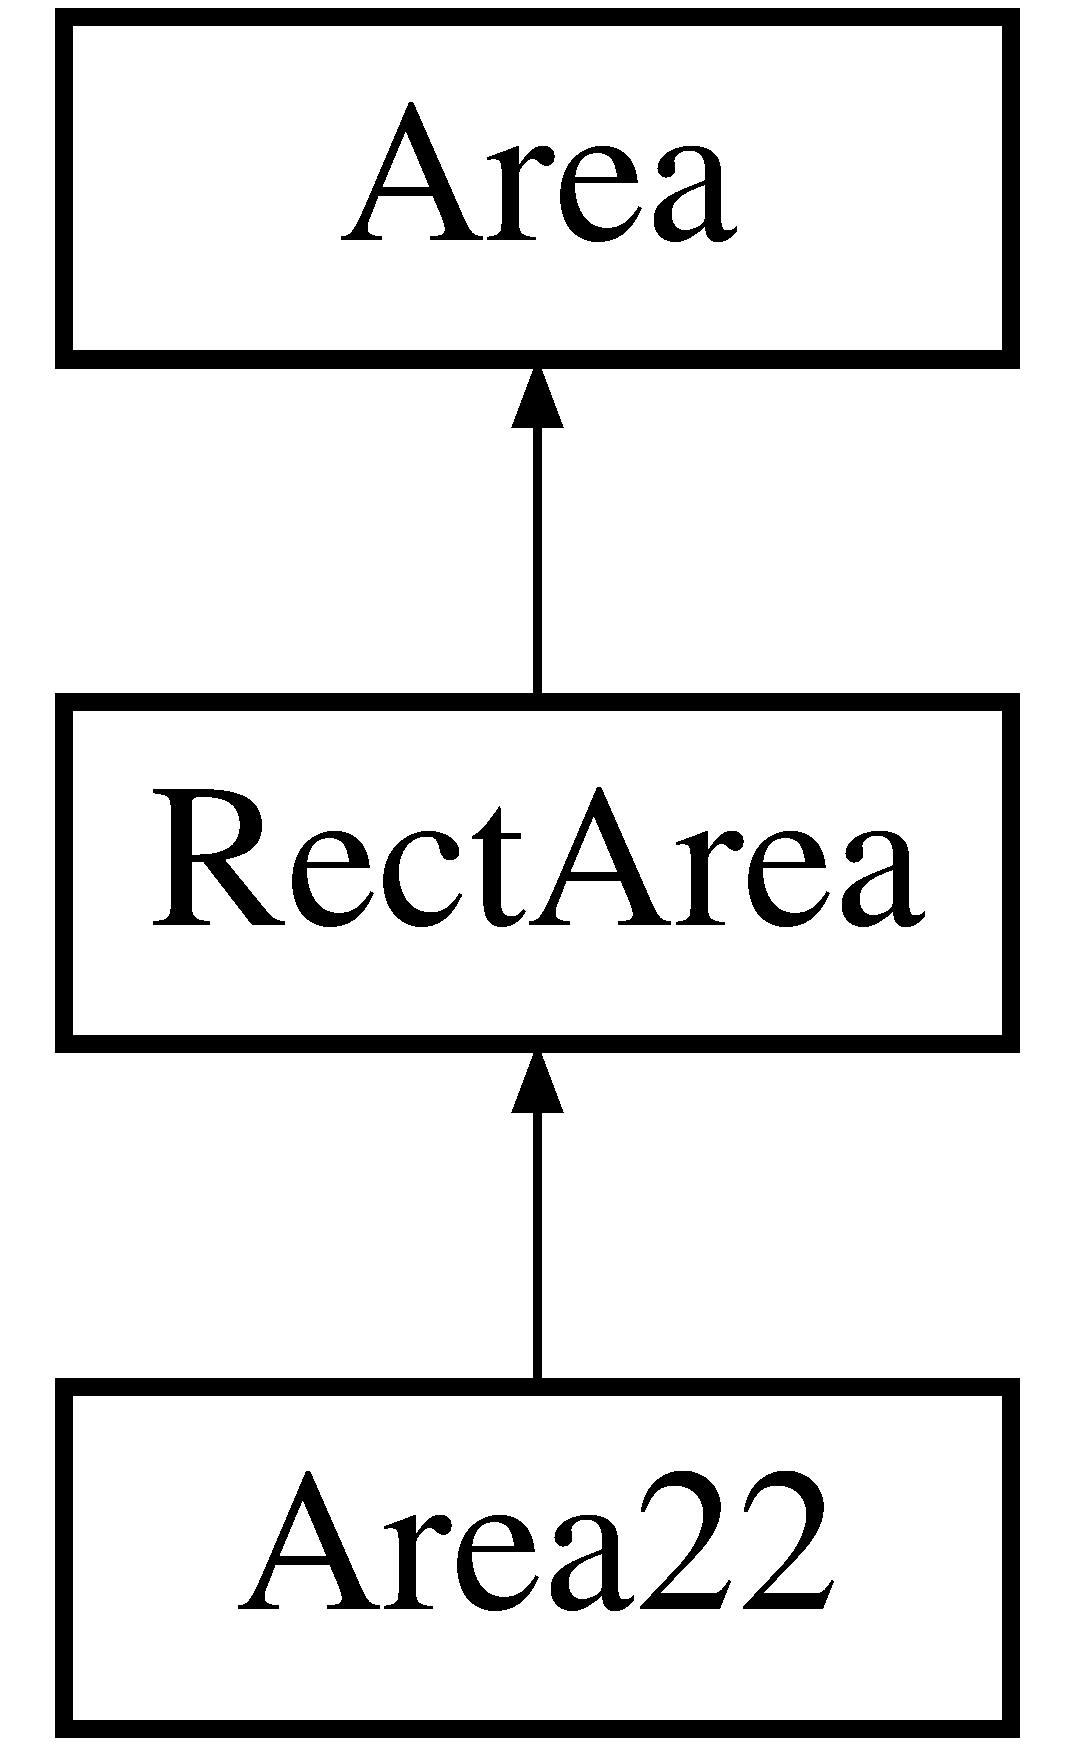
\includegraphics[height=3.000000cm]{class_area22}
\end{center}
\end{figure}
\subsection*{Public Member Functions}
\begin{DoxyCompactItemize}
\item 
\mbox{\Hypertarget{class_area22_a8b5b011a3fdf3c71a8d495edc7640c4b}\label{class_area22_a8b5b011a3fdf3c71a8d495edc7640c4b}} 
{\bfseries Area22} (int n=3, std\+::vector$<$ double $>$ dot=\{ 2, 5, 2, 5, 2, 5 \})
\end{DoxyCompactItemize}
\subsection*{Additional Inherited Members}


The documentation for this class was generated from the following file\+:\begin{DoxyCompactItemize}
\item 
Area.\+h\end{DoxyCompactItemize}

\hypertarget{class_area23}{}\section{Area23 Class Reference}
\label{class_area23}\index{Area23@{Area23}}
Inheritance diagram for Area23\+:\begin{figure}[H]
\begin{center}
\leavevmode
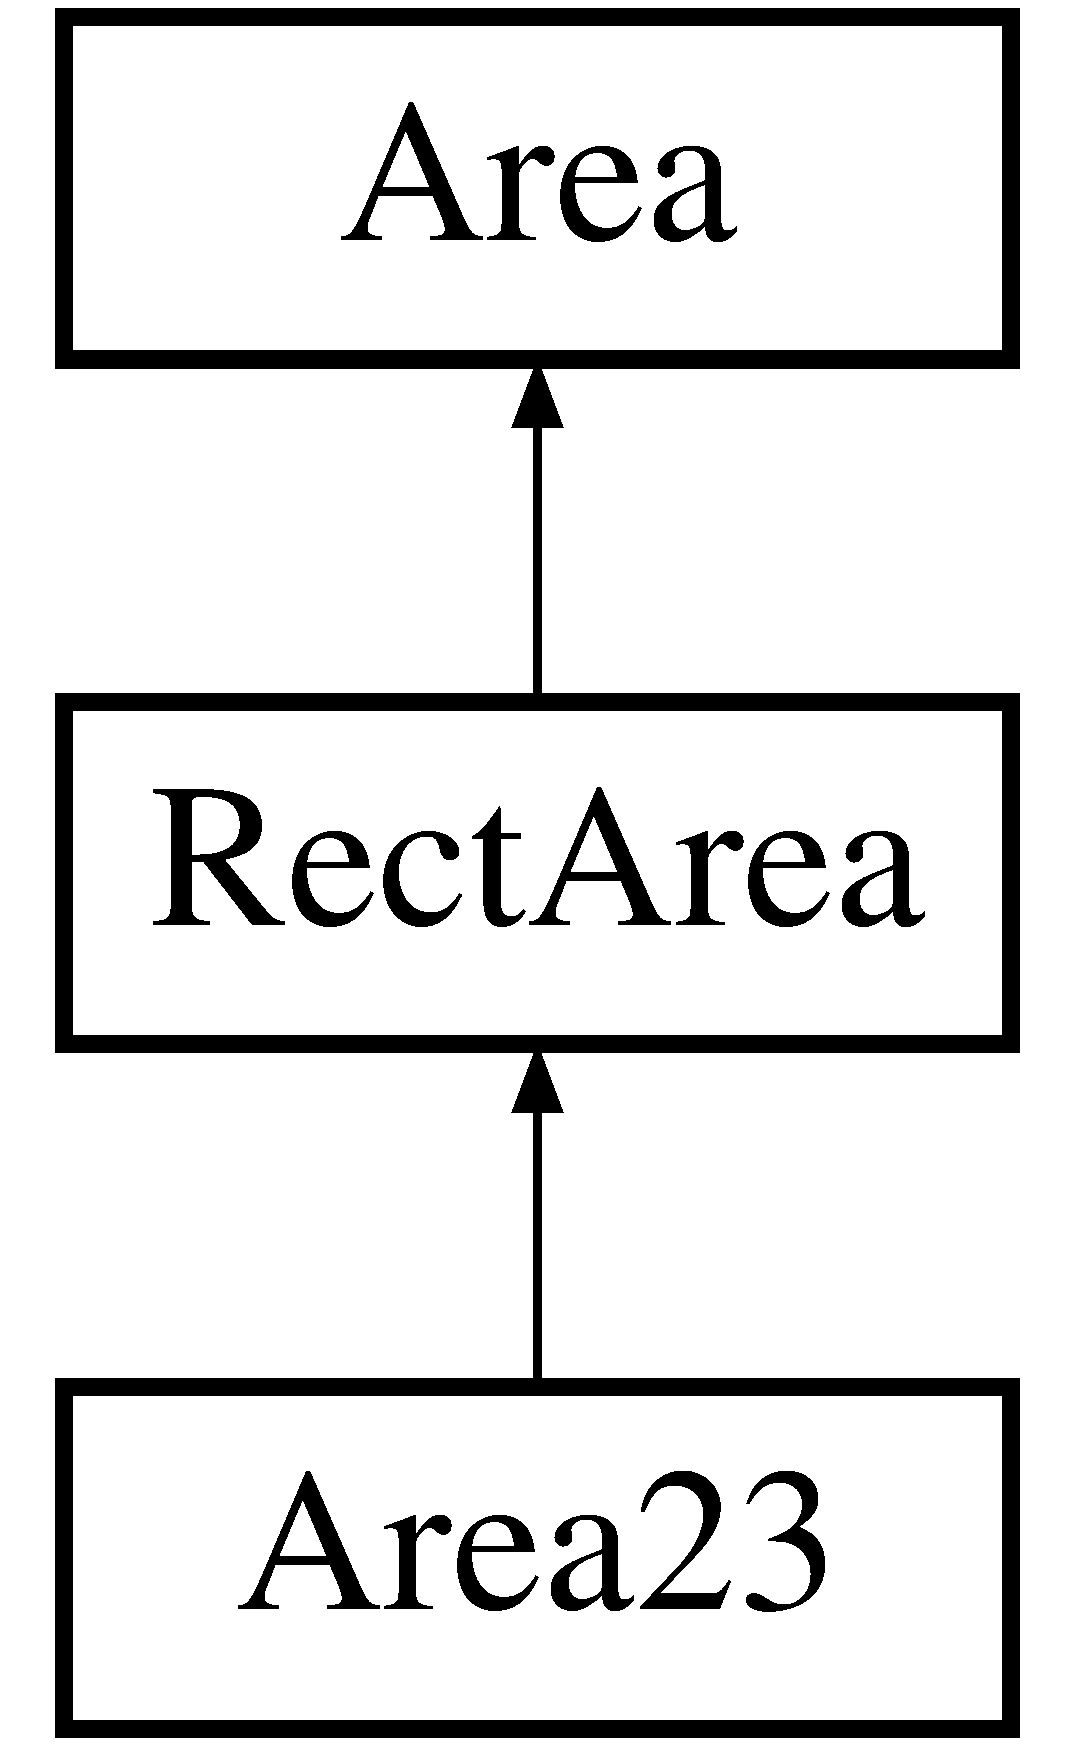
\includegraphics[height=3.000000cm]{class_area23}
\end{center}
\end{figure}
\subsection*{Public Member Functions}
\begin{DoxyCompactItemize}
\item 
\mbox{\Hypertarget{class_area23_aaa474bc086be4c43ef022ddcae50cda1}\label{class_area23_aaa474bc086be4c43ef022ddcae50cda1}} 
{\bfseries Area23} (int n=3, std\+::vector$<$ double $>$ dot=\{ -\/5, 5, -\/5, 5, -\/5, 5 \})
\end{DoxyCompactItemize}
\subsection*{Additional Inherited Members}


The documentation for this class was generated from the following file\+:\begin{DoxyCompactItemize}
\item 
Area.\+h\end{DoxyCompactItemize}

\hypertarget{class_area31}{}\section{Area31 Class Reference}
\label{class_area31}\index{Area31@{Area31}}
Inheritance diagram for Area31\+:\begin{figure}[H]
\begin{center}
\leavevmode
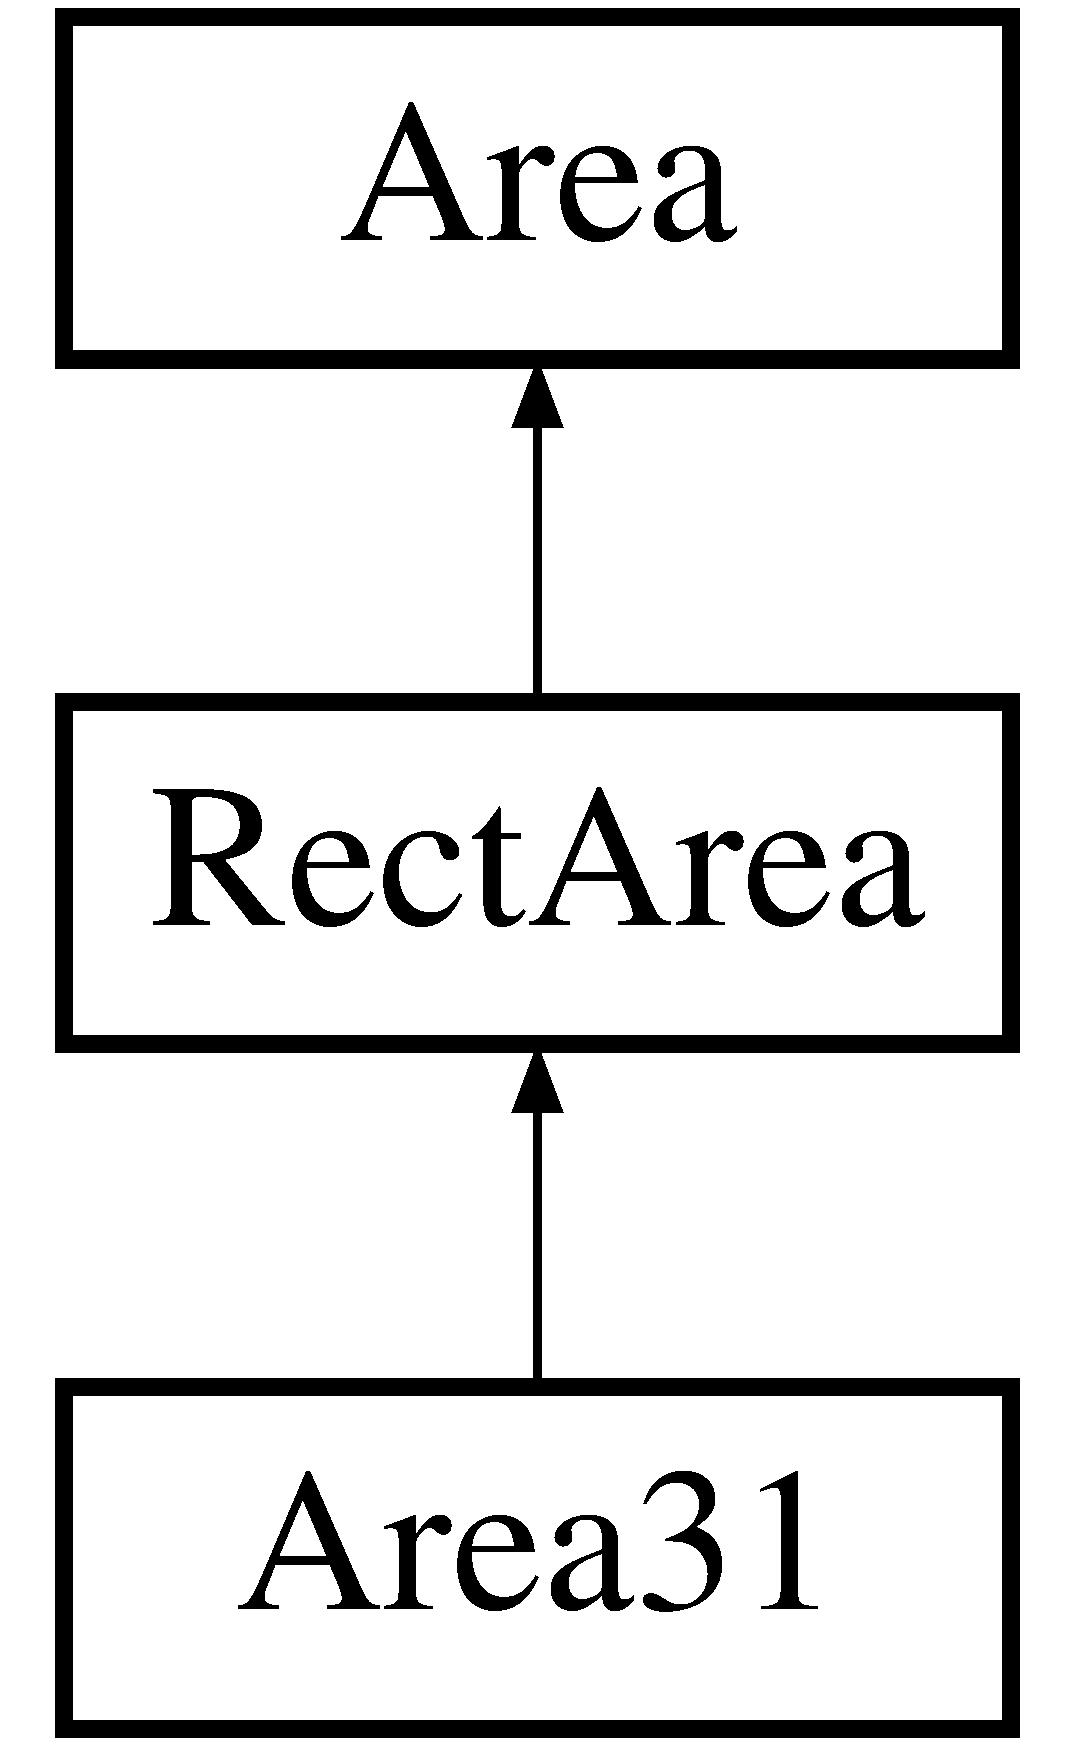
\includegraphics[height=3.000000cm]{class_area31}
\end{center}
\end{figure}
\subsection*{Public Member Functions}
\begin{DoxyCompactItemize}
\item 
\mbox{\Hypertarget{class_area31_a9fe381a6d26ff98208c41e474861509a}\label{class_area31_a9fe381a6d26ff98208c41e474861509a}} 
{\bfseries Area31} (int n=4, std\+::vector$<$ double $>$ dot=\{ 0, 3, 0, 3, 0, 3, 0, 3 \})
\end{DoxyCompactItemize}
\subsection*{Additional Inherited Members}


The documentation for this class was generated from the following file\+:\begin{DoxyCompactItemize}
\item 
Area.\+h\end{DoxyCompactItemize}

\hypertarget{class_area32}{}\section{Area32 Class Reference}
\label{class_area32}\index{Area32@{Area32}}
Inheritance diagram for Area32\+:\begin{figure}[H]
\begin{center}
\leavevmode
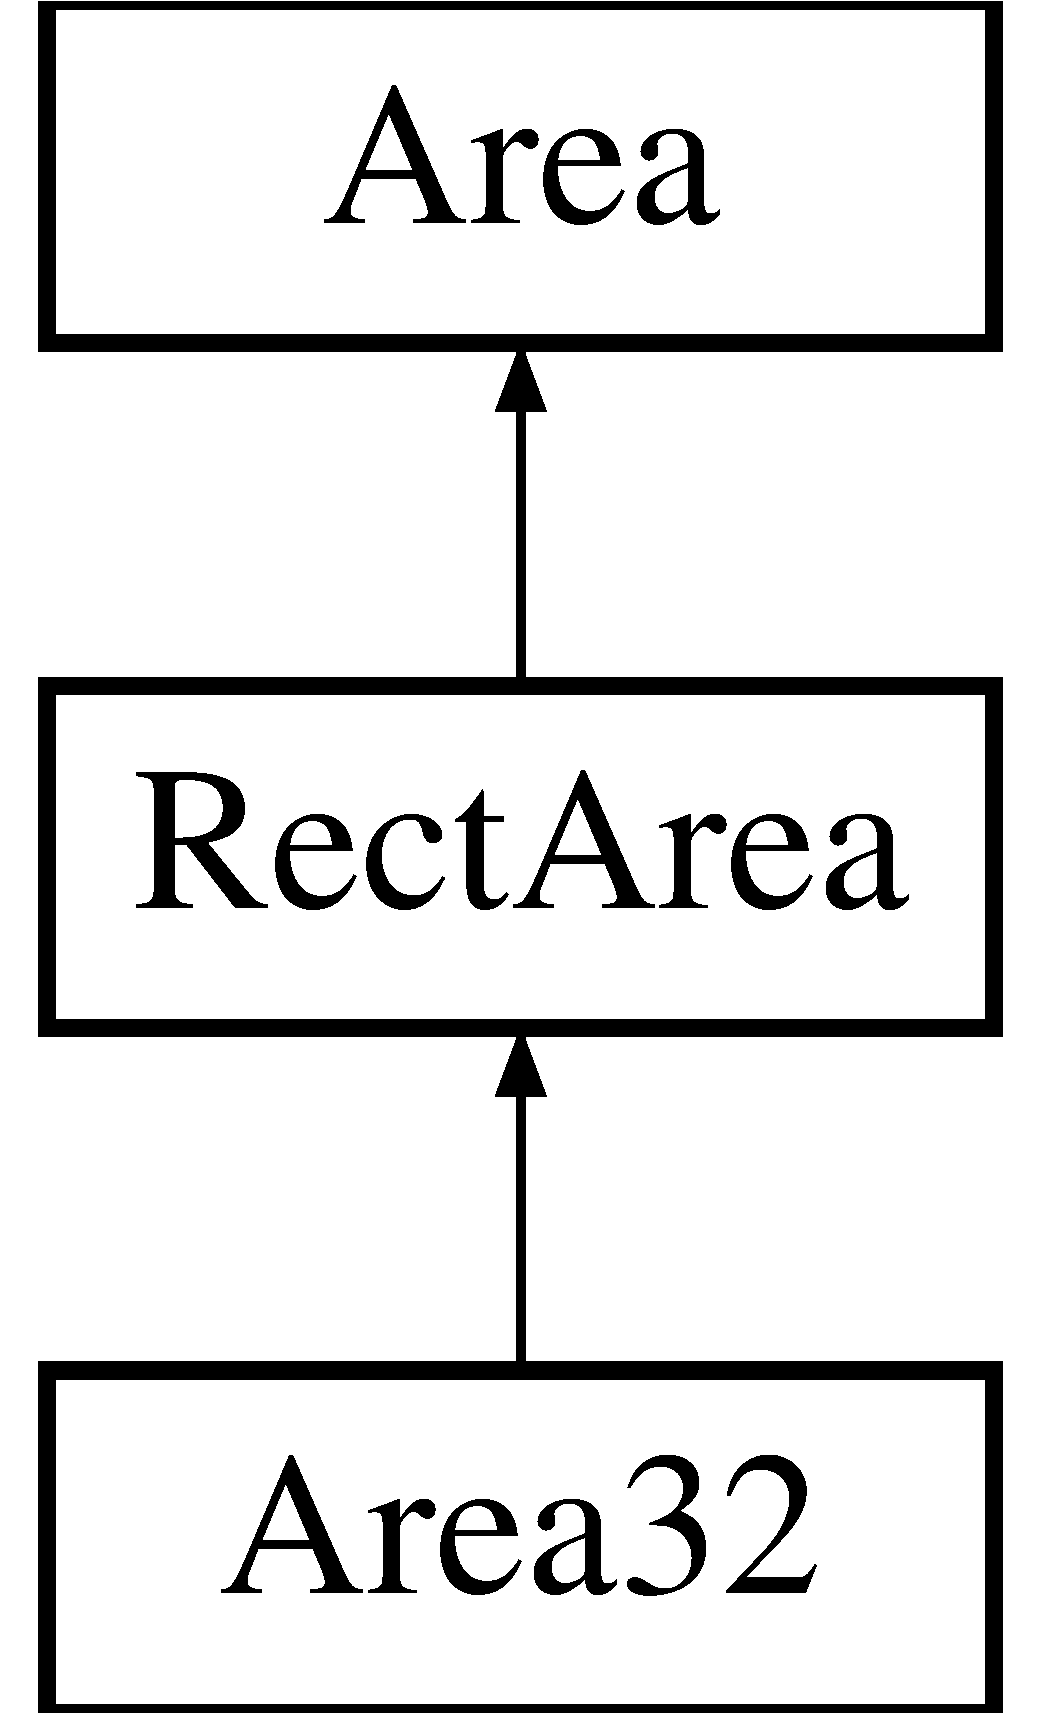
\includegraphics[height=3.000000cm]{class_area32}
\end{center}
\end{figure}
\subsection*{Public Member Functions}
\begin{DoxyCompactItemize}
\item 
\mbox{\Hypertarget{class_area32_a8d99e0e27d2f86097a5ff4ea03e9503d}\label{class_area32_a8d99e0e27d2f86097a5ff4ea03e9503d}} 
{\bfseries Area32} (int n=4, std\+::vector$<$ double $>$ dot=\{ 2, 5, 2, 5, 2, 5, 2, 5 \})
\end{DoxyCompactItemize}
\subsection*{Additional Inherited Members}


The documentation for this class was generated from the following file\+:\begin{DoxyCompactItemize}
\item 
Area.\+h\end{DoxyCompactItemize}

\hypertarget{class_area33}{}\section{Area33 Class Reference}
\label{class_area33}\index{Area33@{Area33}}
Inheritance diagram for Area33\+:\begin{figure}[H]
\begin{center}
\leavevmode
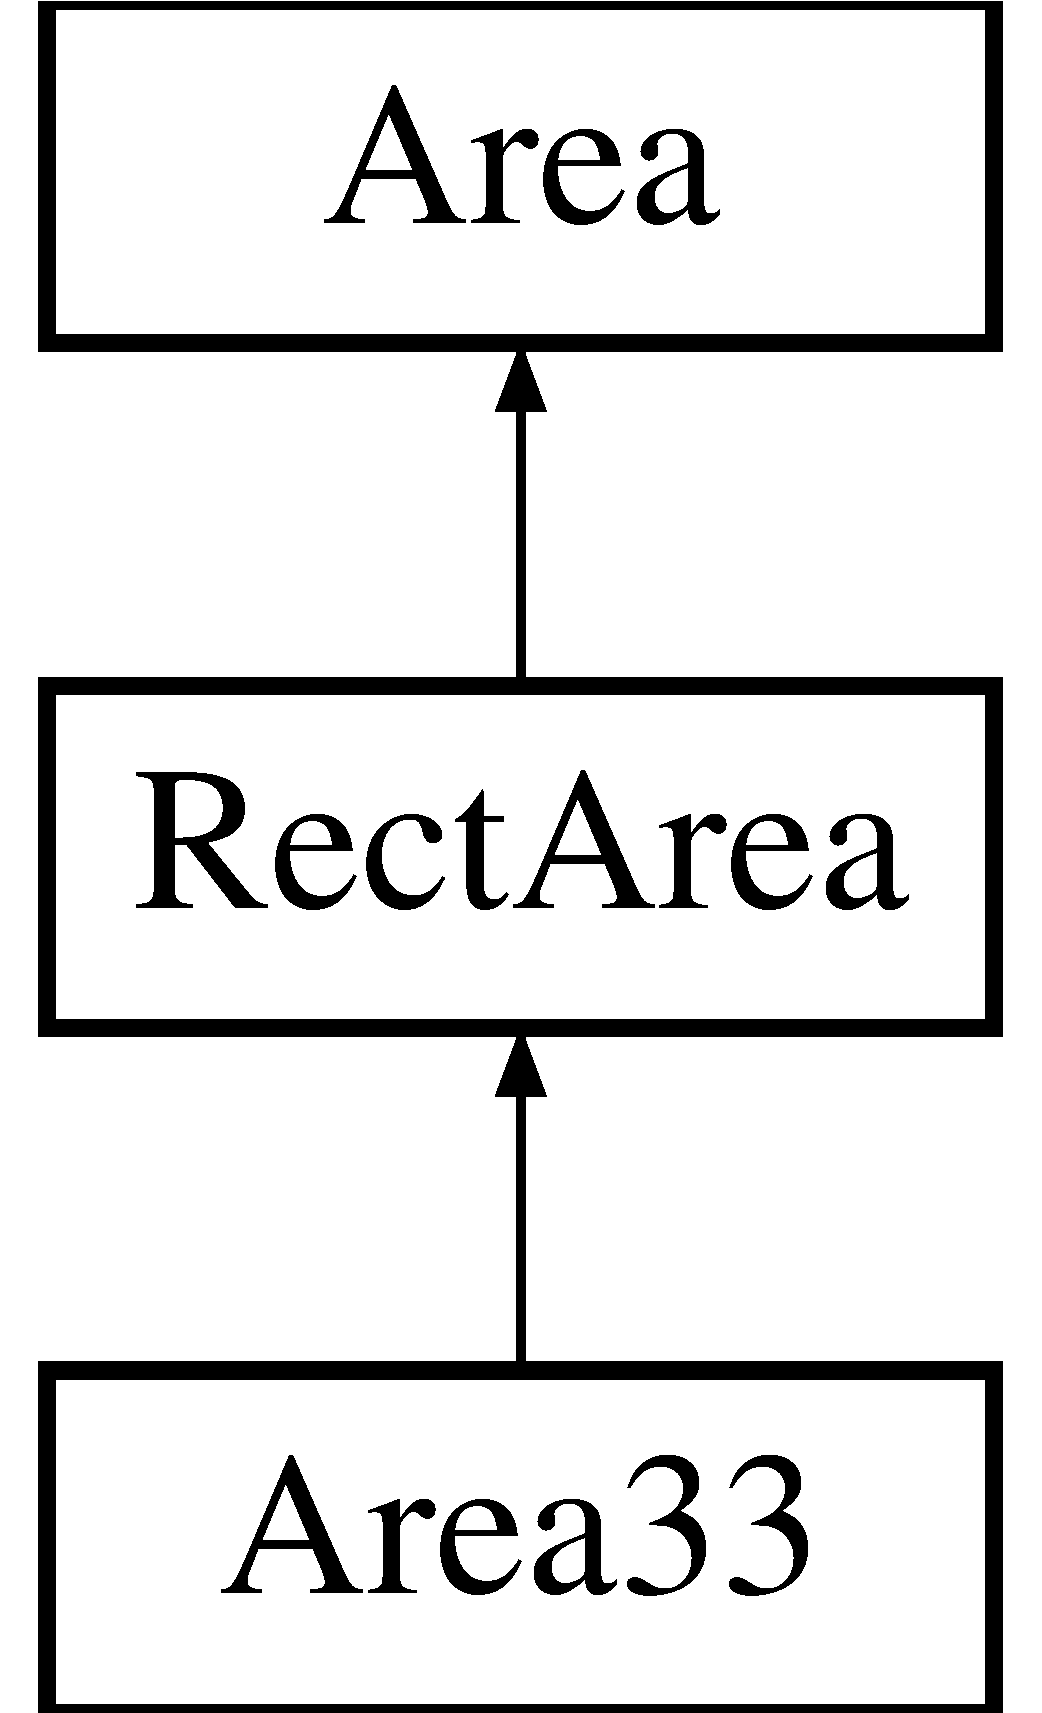
\includegraphics[height=3.000000cm]{class_area33}
\end{center}
\end{figure}
\subsection*{Public Member Functions}
\begin{DoxyCompactItemize}
\item 
\mbox{\Hypertarget{class_area33_a9e02db1a6fcdc9479f6b0c35bf6b6c67}\label{class_area33_a9e02db1a6fcdc9479f6b0c35bf6b6c67}} 
{\bfseries Area33} (int n=4, std\+::vector$<$ double $>$ dot=\{ -\/5, 5, -\/5, 5, -\/5, 5, -\/5, 5 \})
\end{DoxyCompactItemize}
\subsection*{Additional Inherited Members}


The documentation for this class was generated from the following file\+:\begin{DoxyCompactItemize}
\item 
Area.\+h\end{DoxyCompactItemize}

\hypertarget{classcoord}{}\section{coord Class Reference}
\label{classcoord}\index{coord@{coord}}
Inheritance diagram for coord\+:\begin{figure}[H]
\begin{center}
\leavevmode
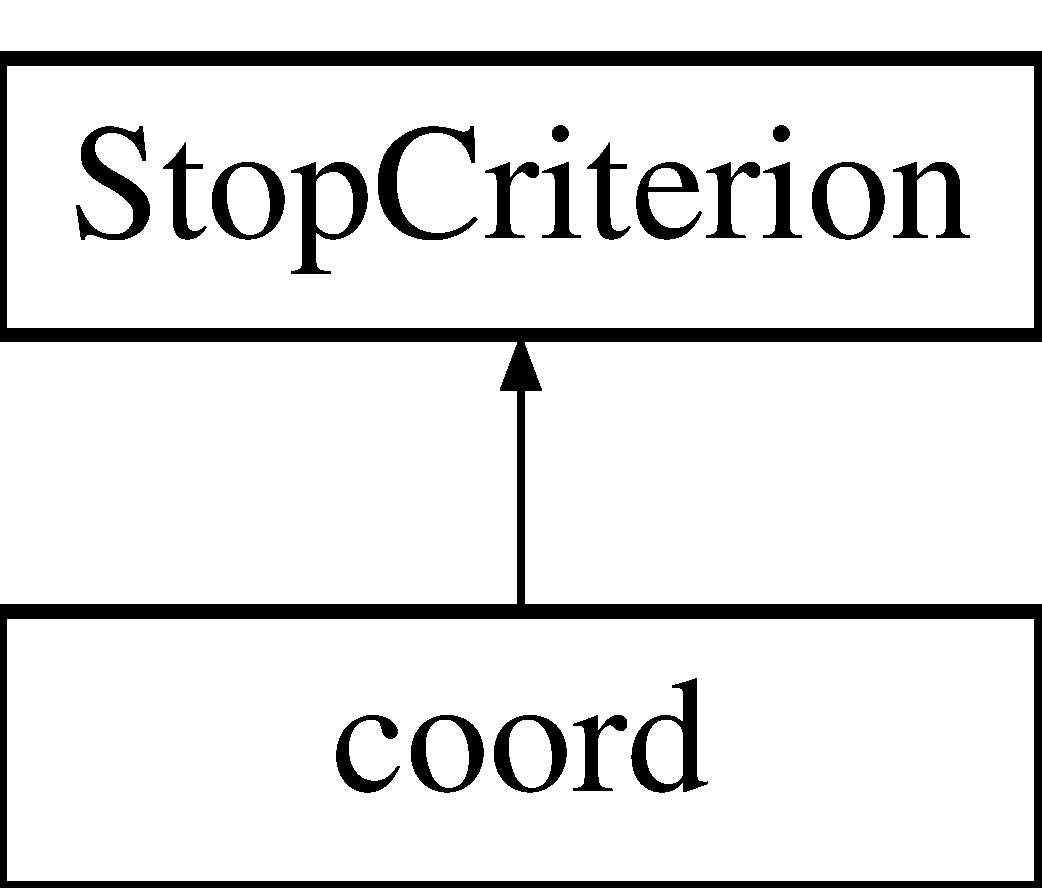
\includegraphics[height=2.000000cm]{classcoord}
\end{center}
\end{figure}
\subsection*{Public Member Functions}
\begin{DoxyCompactItemize}
\item 
\mbox{\Hypertarget{classcoord_a7a339b16b6173691c9fd8d6b7485144f}\label{classcoord_a7a339b16b6173691c9fd8d6b7485144f}} 
virtual bool \mbox{\hyperlink{classcoord_a7a339b16b6173691c9fd8d6b7485144f}{stop}} (std\+::vector$<$ double $>$ x0, std\+::vector$<$ double $>$ x1, double f0, double f1, std\+::vector$<$ double $>$ grad) override
\begin{DoxyCompactList}\small\item\em Функция, осуществляющая проверку выбранного критерия остановки и возвращающая соответсвующее значение \end{DoxyCompactList}\end{DoxyCompactItemize}
\subsection*{Additional Inherited Members}


The documentation for this class was generated from the following files\+:\begin{DoxyCompactItemize}
\item 
Stop\+Criterion.\+h\item 
Stop\+Criterion.\+cpp\end{DoxyCompactItemize}

\hypertarget{class_fletcher_reeves_c_g}{}\section{Fletcher\+Reeves\+CG Class Reference}
\label{class_fletcher_reeves_c_g}\index{Fletcher\+Reeves\+CG@{Fletcher\+Reeves\+CG}}
Inheritance diagram for Fletcher\+Reeves\+CG\+:\begin{figure}[H]
\begin{center}
\leavevmode
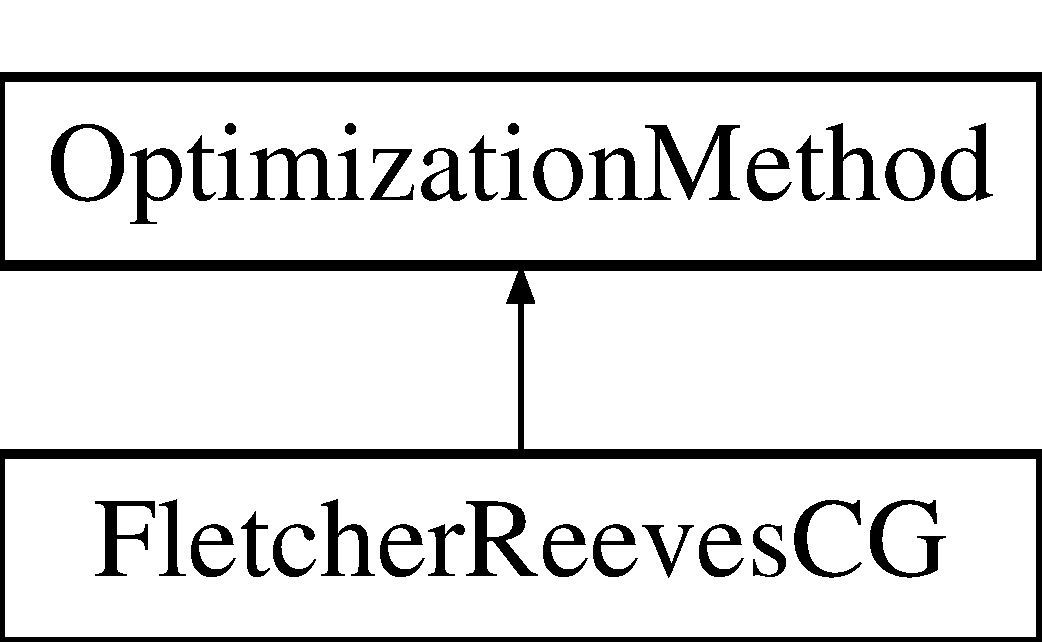
\includegraphics[height=2.000000cm]{class_fletcher_reeves_c_g}
\end{center}
\end{figure}
\subsection*{Public Member Functions}
\begin{DoxyCompactItemize}
\item 
virtual std\+::vector$<$ double $>$ \mbox{\hyperlink{class_fletcher_reeves_c_g_a40c56c0485371b31000672236b433dc7}{optimize}} (\mbox{\hyperlink{class_area}{Area}} $\ast$area, \mbox{\hyperlink{class_function}{Function}} $\ast$func, \mbox{\hyperlink{class_stop_criterion}{Stop\+Criterion}} $\ast$criterion) override
\end{DoxyCompactItemize}
\subsection*{Additional Inherited Members}


\subsection{Member Function Documentation}
\mbox{\Hypertarget{class_fletcher_reeves_c_g_a40c56c0485371b31000672236b433dc7}\label{class_fletcher_reeves_c_g_a40c56c0485371b31000672236b433dc7}} 
\index{Fletcher\+Reeves\+CG@{Fletcher\+Reeves\+CG}!optimize@{optimize}}
\index{optimize@{optimize}!Fletcher\+Reeves\+CG@{Fletcher\+Reeves\+CG}}
\subsubsection{\texorpdfstring{optimize()}{optimize()}}
{\footnotesize\ttfamily std\+::vector$<$ double $>$ Fletcher\+Reeves\+C\+G\+::optimize (\begin{DoxyParamCaption}\item[{\mbox{\hyperlink{class_area}{Area}} $\ast$}]{area,  }\item[{\mbox{\hyperlink{class_function}{Function}} $\ast$}]{func,  }\item[{\mbox{\hyperlink{class_stop_criterion}{Stop\+Criterion}} $\ast$}]{criterion }\end{DoxyParamCaption})\hspace{0.3cm}{\ttfamily [override]}, {\ttfamily [virtual]}}

Функция нахождения минимума функции и точки, в которой он достигается 
\begin{DoxyParams}{Parameters}
{\em area} & Выбранная область, в которой будет находиться минимум \\
\hline
{\em func} & Функция, минимум которой будет находиться \\
\hline
{\em criterion} & Критерий остановки для выбранного метода \\
\hline
\end{DoxyParams}
\begin{DoxyReturn}{Returns}
Точку минимума функции в области 
\end{DoxyReturn}


Implements \mbox{\hyperlink{class_optimization_method_a63dd17c00593363a017c8dd440770aa2}{Optimization\+Method}}.



The documentation for this class was generated from the following files\+:\begin{DoxyCompactItemize}
\item 
Optimization\+Method.\+h\item 
Optimization\+Method.\+cpp\end{DoxyCompactItemize}

\hypertarget{class_function}{}\section{Function Class Reference}
\label{class_function}\index{Function@{Function}}


{\ttfamily \#include $<$Function.\+h$>$}

Inheritance diagram for Function\+:\begin{figure}[H]
\begin{center}
\leavevmode
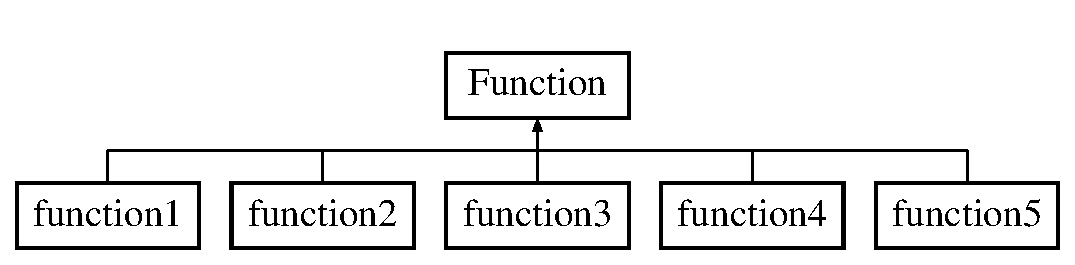
\includegraphics[height=2.000000cm]{class_function}
\end{center}
\end{figure}
\subsection*{Public Member Functions}
\begin{DoxyCompactItemize}
\item 
\mbox{\Hypertarget{class_function_a718c397736583f381104e7eb5cc25d49}\label{class_function_a718c397736583f381104e7eb5cc25d49}} 
virtual double \mbox{\hyperlink{class_function_a718c397736583f381104e7eb5cc25d49}{eval}} (std\+::vector$<$ double $>$ x)=0
\begin{DoxyCompactList}\small\item\em Вычисляет выбранную ффункцию в заданной точке \end{DoxyCompactList}\item 
\mbox{\Hypertarget{class_function_aa160e1771be2c8724eb32e6d841a2d37}\label{class_function_aa160e1771be2c8724eb32e6d841a2d37}} 
std\+::vector$<$ double $>$ \mbox{\hyperlink{class_function_aa160e1771be2c8724eb32e6d841a2d37}{minus\+\_\+eval\+\_\+grad}} (std\+::vector$<$ double $>$ x)
\begin{DoxyCompactList}\small\item\em Вычисляет градиент со знаком минус выбранной функции в заданной точке \end{DoxyCompactList}\item 
\mbox{\Hypertarget{class_function_aabb9556d29e6899785a2cbacad2901ea}\label{class_function_aabb9556d29e6899785a2cbacad2901ea}} 
void {\bfseries Set\+\_\+eps} (double epsil)
\end{DoxyCompactItemize}
\subsection*{Protected Attributes}
\begin{DoxyCompactItemize}
\item 
\mbox{\Hypertarget{class_function_a8c8efa0bbf1e627367b7a4bc02b5a5ce}\label{class_function_a8c8efa0bbf1e627367b7a4bc02b5a5ce}} 
double {\bfseries eps}
\end{DoxyCompactItemize}


\subsection{Detailed Description}
Данный класс содержит определения заданных функций, предоставляемых на выбор пользователю. 

The documentation for this class was generated from the following files\+:\begin{DoxyCompactItemize}
\item 
Function.\+h\item 
Function.\+cpp\end{DoxyCompactItemize}

\hypertarget{classfunction1}{}\section{function1 Class Reference}
\label{classfunction1}\index{function1@{function1}}
Inheritance diagram for function1\+:\begin{figure}[H]
\begin{center}
\leavevmode
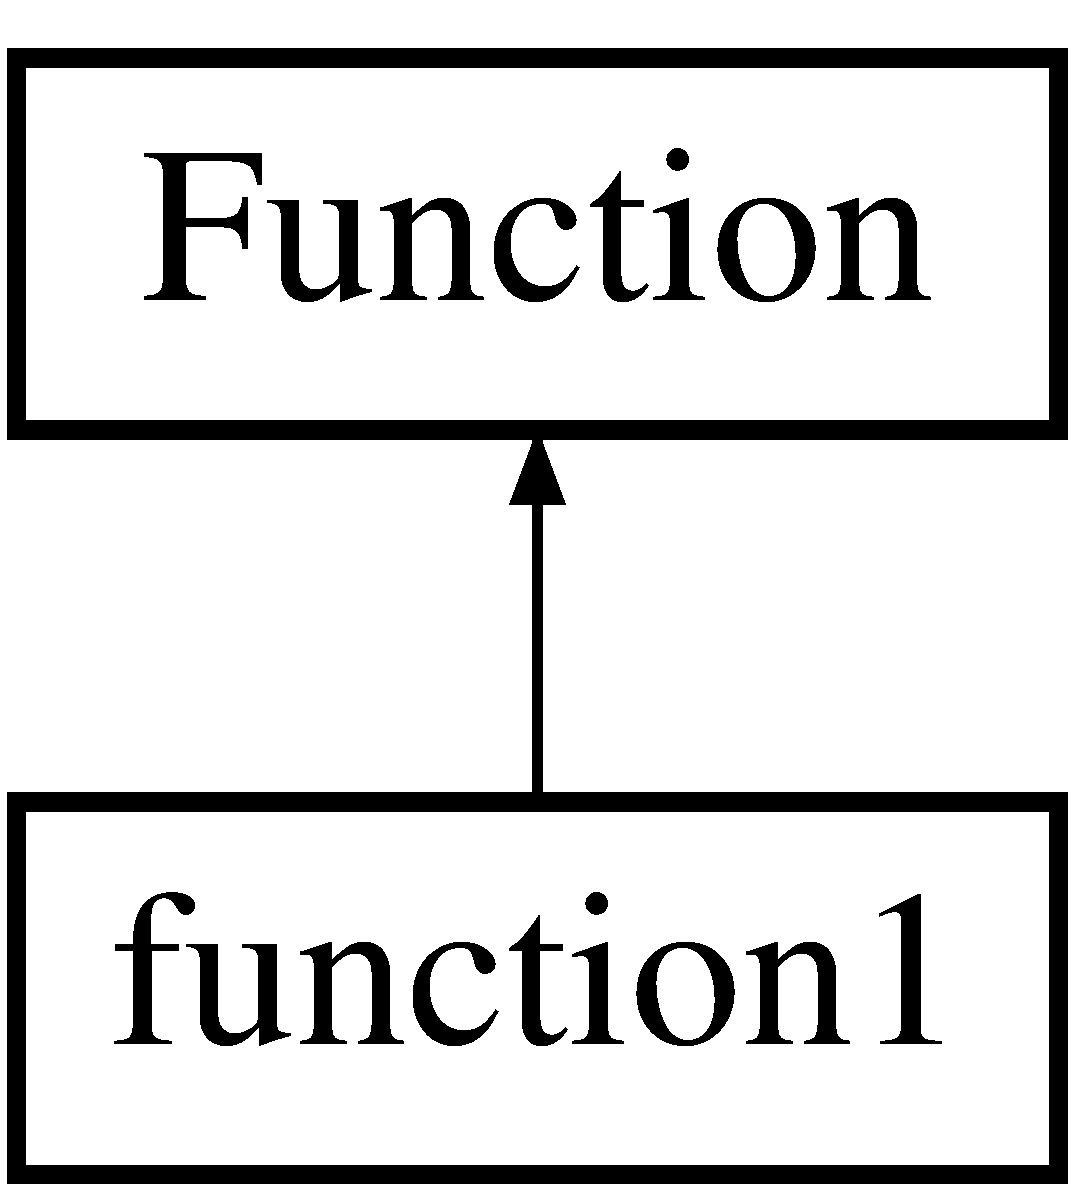
\includegraphics[height=2.000000cm]{classfunction1}
\end{center}
\end{figure}
\subsection*{Public Member Functions}
\begin{DoxyCompactItemize}
\item 
\mbox{\Hypertarget{classfunction1_afcf1eb63c3348dfc970d7e439d7386c9}\label{classfunction1_afcf1eb63c3348dfc970d7e439d7386c9}} 
virtual double \mbox{\hyperlink{classfunction1_afcf1eb63c3348dfc970d7e439d7386c9}{eval}} (std\+::vector$<$ double $>$ x) override
\begin{DoxyCompactList}\small\item\em Вычисляет выбранную ффункцию в заданной точке \end{DoxyCompactList}\end{DoxyCompactItemize}
\subsection*{Additional Inherited Members}


The documentation for this class was generated from the following files\+:\begin{DoxyCompactItemize}
\item 
Function.\+h\item 
Function.\+cpp\end{DoxyCompactItemize}

\hypertarget{classfunction2}{}\section{function2 Class Reference}
\label{classfunction2}\index{function2@{function2}}
Inheritance diagram for function2\+:\begin{figure}[H]
\begin{center}
\leavevmode
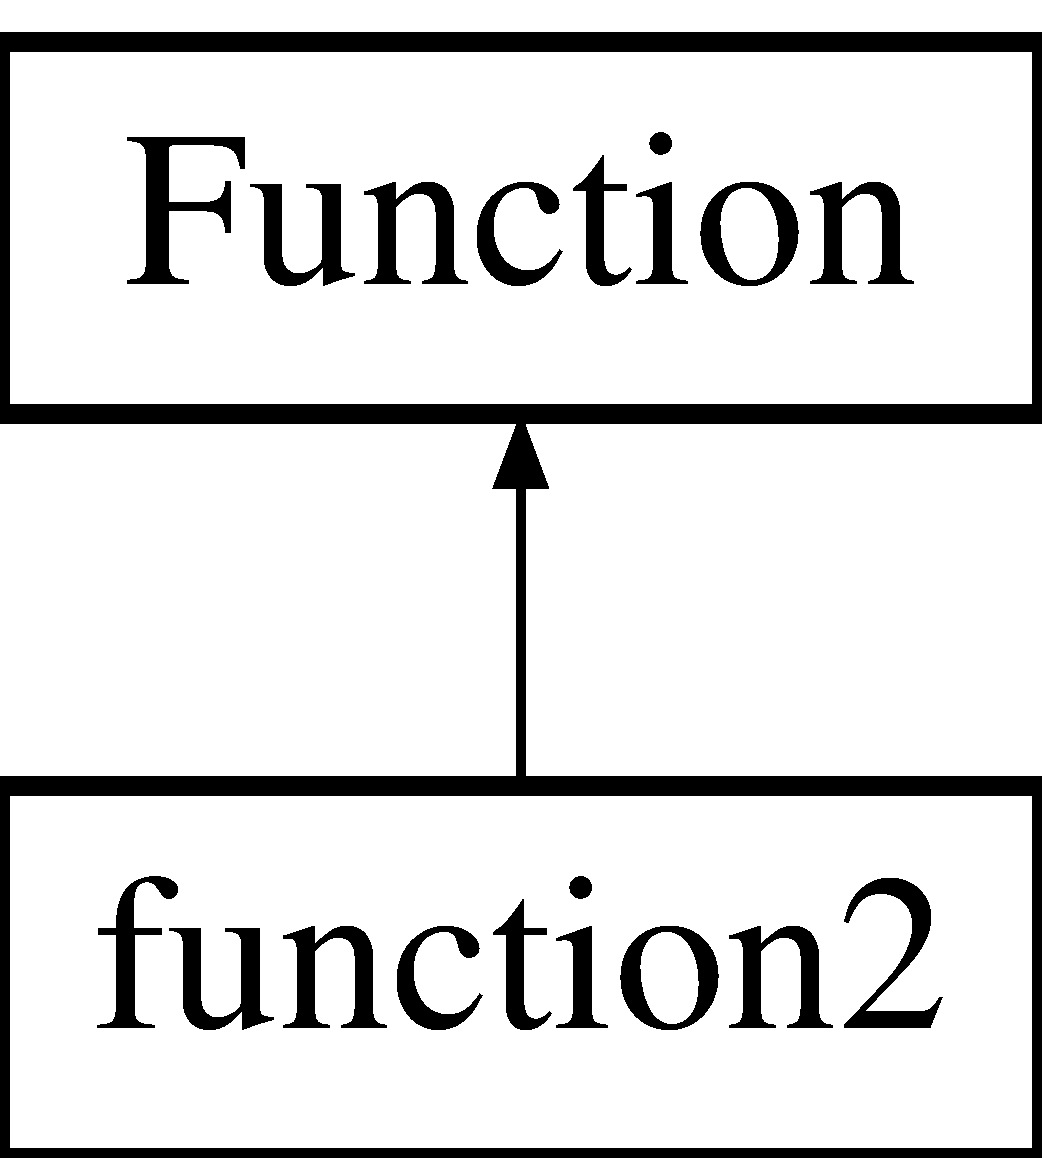
\includegraphics[height=2.000000cm]{classfunction2}
\end{center}
\end{figure}
\subsection*{Public Member Functions}
\begin{DoxyCompactItemize}
\item 
\mbox{\Hypertarget{classfunction2_a025422903184307ecb17181cec02c79a}\label{classfunction2_a025422903184307ecb17181cec02c79a}} 
virtual double \mbox{\hyperlink{classfunction2_a025422903184307ecb17181cec02c79a}{eval}} (std\+::vector$<$ double $>$ x) override
\begin{DoxyCompactList}\small\item\em Вычисляет выбранную ффункцию в заданной точке \end{DoxyCompactList}\end{DoxyCompactItemize}
\subsection*{Additional Inherited Members}


The documentation for this class was generated from the following files\+:\begin{DoxyCompactItemize}
\item 
Function.\+h\item 
Function.\+cpp\end{DoxyCompactItemize}

\hypertarget{classfunction3}{}\section{function3 Class Reference}
\label{classfunction3}\index{function3@{function3}}
Inheritance diagram for function3\+:\begin{figure}[H]
\begin{center}
\leavevmode
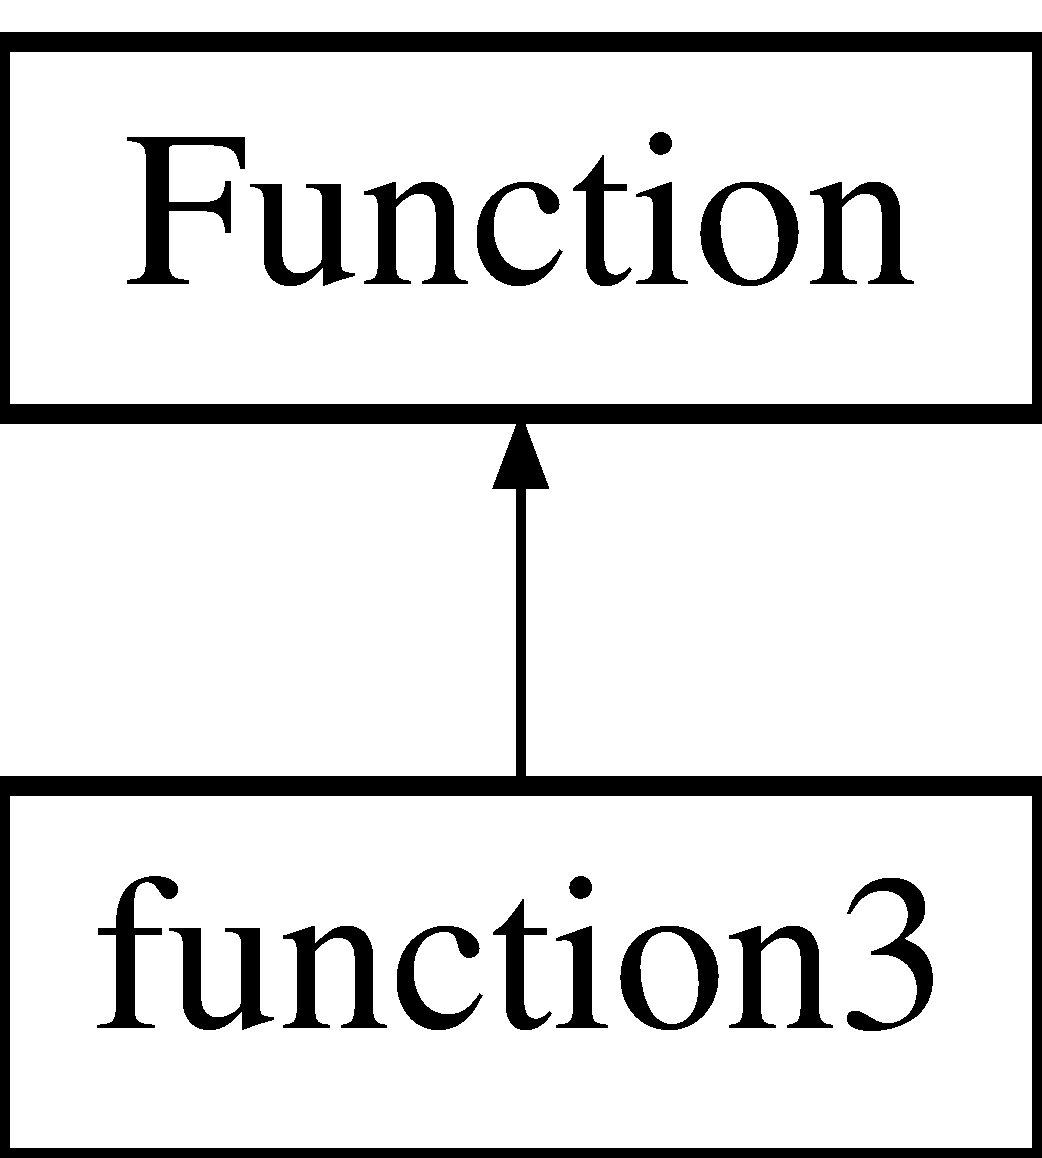
\includegraphics[height=2.000000cm]{classfunction3}
\end{center}
\end{figure}
\subsection*{Public Member Functions}
\begin{DoxyCompactItemize}
\item 
\mbox{\Hypertarget{classfunction3_aeeb95e4688599d08134d56f51cdf4268}\label{classfunction3_aeeb95e4688599d08134d56f51cdf4268}} 
virtual double \mbox{\hyperlink{classfunction3_aeeb95e4688599d08134d56f51cdf4268}{eval}} (std\+::vector$<$ double $>$ x) override
\begin{DoxyCompactList}\small\item\em Вычисляет выбранную ффункцию в заданной точке \end{DoxyCompactList}\end{DoxyCompactItemize}
\subsection*{Additional Inherited Members}


The documentation for this class was generated from the following files\+:\begin{DoxyCompactItemize}
\item 
Function.\+h\item 
Function.\+cpp\end{DoxyCompactItemize}

\hypertarget{classfunction4}{}\section{function4 Class Reference}
\label{classfunction4}\index{function4@{function4}}
Inheritance diagram for function4\+:\begin{figure}[H]
\begin{center}
\leavevmode
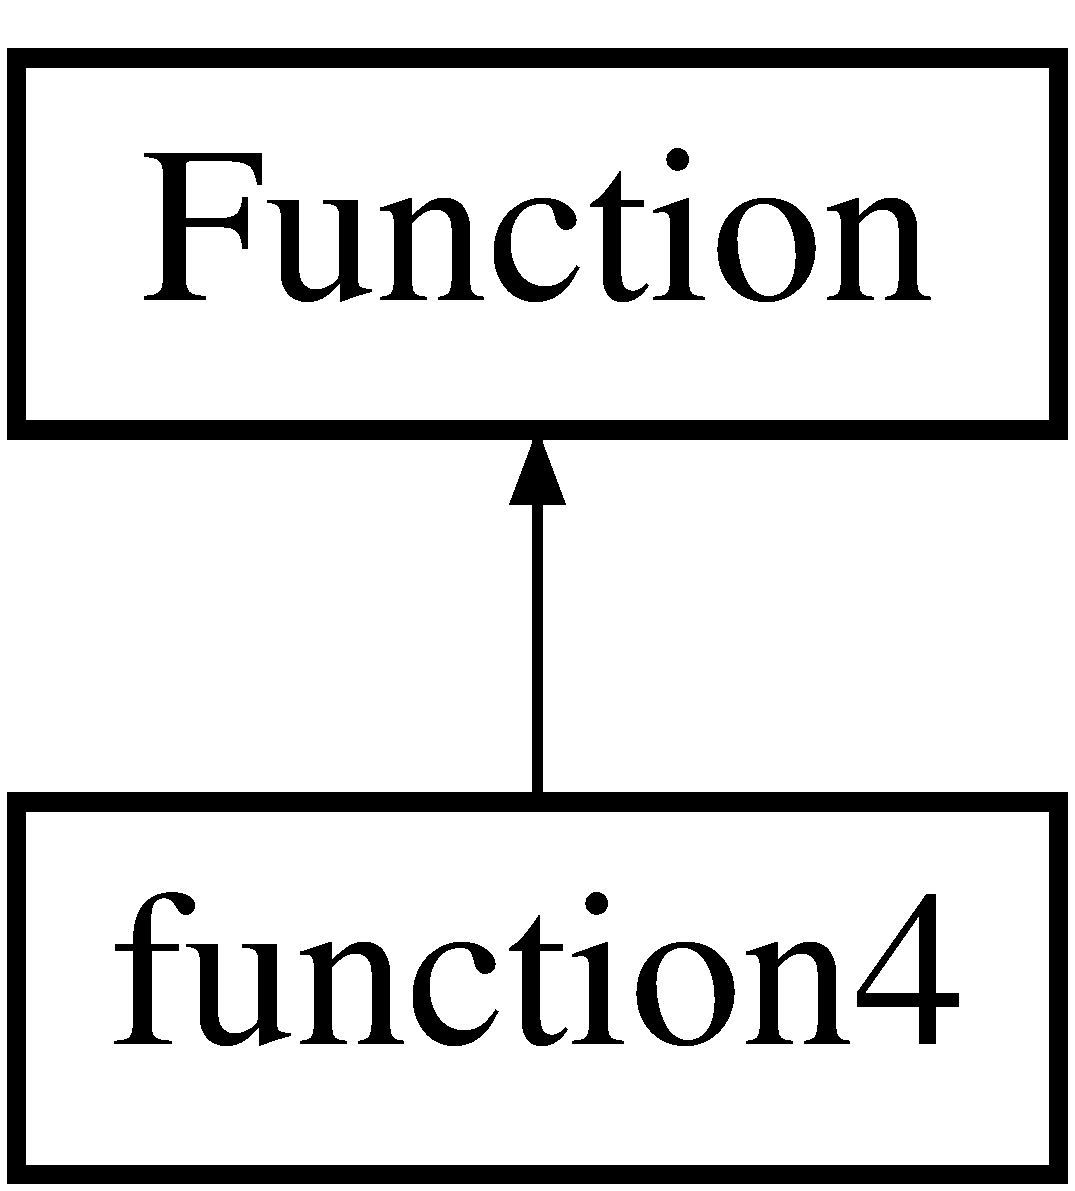
\includegraphics[height=2.000000cm]{classfunction4}
\end{center}
\end{figure}
\subsection*{Public Member Functions}
\begin{DoxyCompactItemize}
\item 
\mbox{\Hypertarget{classfunction4_ab463eeb605f2598995f6d4e42e91fe45}\label{classfunction4_ab463eeb605f2598995f6d4e42e91fe45}} 
virtual double \mbox{\hyperlink{classfunction4_ab463eeb605f2598995f6d4e42e91fe45}{eval}} (std\+::vector$<$ double $>$ x) override
\begin{DoxyCompactList}\small\item\em Вычисляет выбранную ффункцию в заданной точке \end{DoxyCompactList}\end{DoxyCompactItemize}
\subsection*{Additional Inherited Members}


The documentation for this class was generated from the following files\+:\begin{DoxyCompactItemize}
\item 
Function.\+h\item 
Function.\+cpp\end{DoxyCompactItemize}

\hypertarget{classfunction5}{}\section{function5 Class Reference}
\label{classfunction5}\index{function5@{function5}}
Inheritance diagram for function5\+:\begin{figure}[H]
\begin{center}
\leavevmode
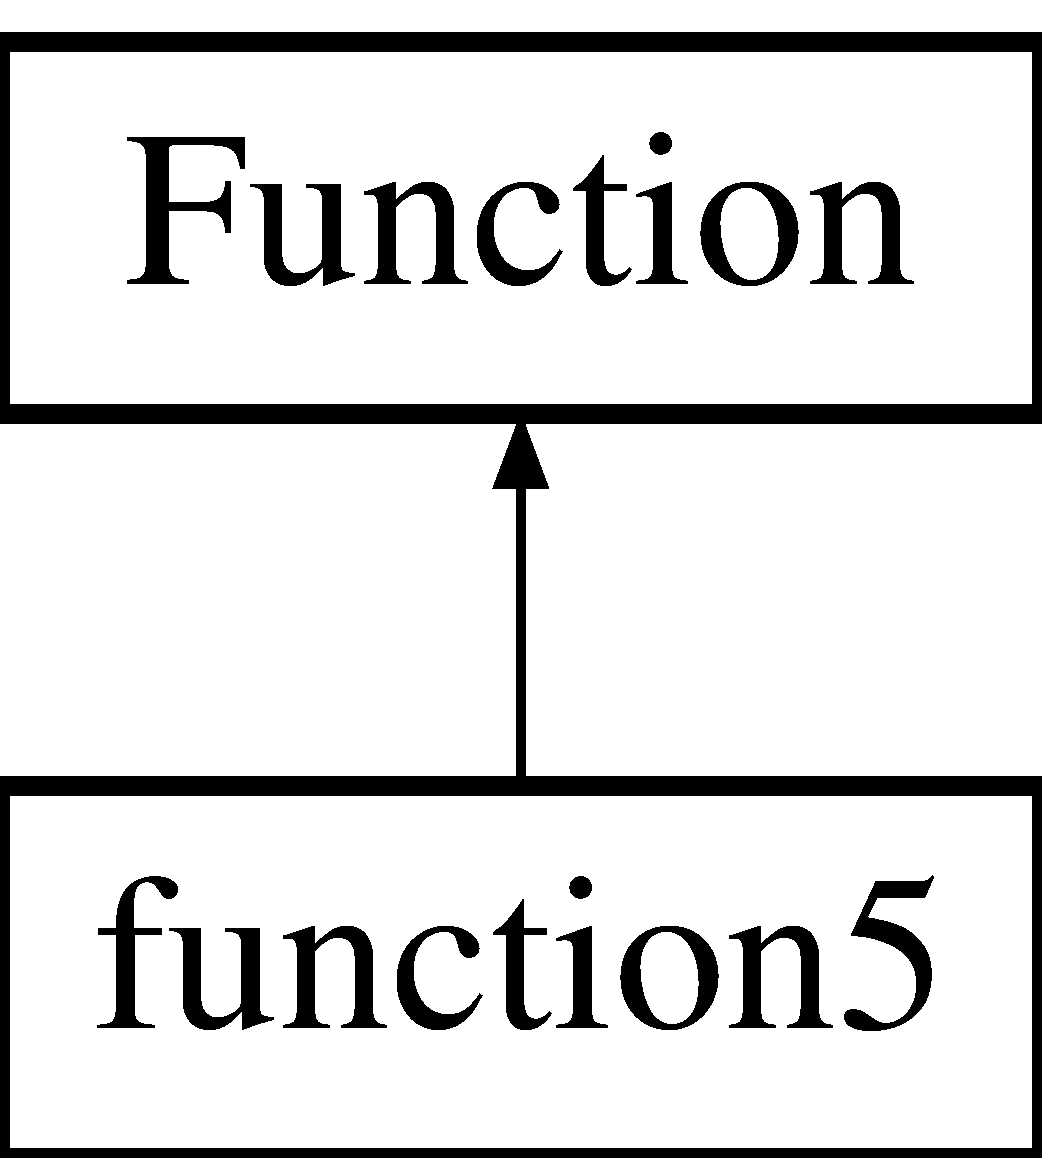
\includegraphics[height=2.000000cm]{classfunction5}
\end{center}
\end{figure}
\subsection*{Public Member Functions}
\begin{DoxyCompactItemize}
\item 
\mbox{\Hypertarget{classfunction5_a3710d7f05bce2203088b8bdd15916dcc}\label{classfunction5_a3710d7f05bce2203088b8bdd15916dcc}} 
virtual double \mbox{\hyperlink{classfunction5_a3710d7f05bce2203088b8bdd15916dcc}{eval}} (std\+::vector$<$ double $>$ x) override
\begin{DoxyCompactList}\small\item\em Вычисляет выбранную ффункцию в заданной точке \end{DoxyCompactList}\end{DoxyCompactItemize}
\subsection*{Additional Inherited Members}


The documentation for this class was generated from the following files\+:\begin{DoxyCompactItemize}
\item 
Function.\+h\item 
Function.\+cpp\end{DoxyCompactItemize}

\hypertarget{classlast__improv}{}\section{last\+\_\+improv Class Reference}
\label{classlast__improv}\index{last\+\_\+improv@{last\+\_\+improv}}
Inheritance diagram for last\+\_\+improv\+:\begin{figure}[H]
\begin{center}
\leavevmode
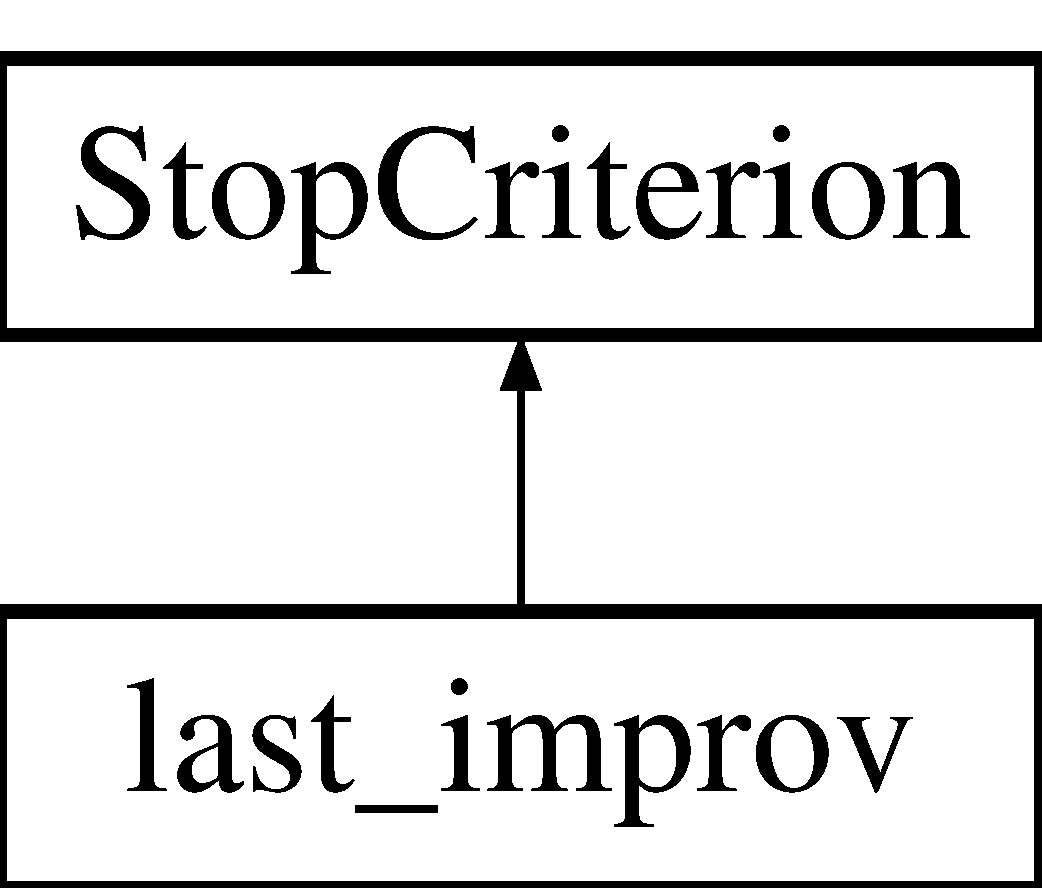
\includegraphics[height=2.000000cm]{classlast__improv}
\end{center}
\end{figure}
\subsection*{Public Member Functions}
\begin{DoxyCompactItemize}
\item 
\mbox{\Hypertarget{classlast__improv_aed14fdf2a6a5c1638a012d9f58f114b7}\label{classlast__improv_aed14fdf2a6a5c1638a012d9f58f114b7}} 
virtual bool \mbox{\hyperlink{classlast__improv_aed14fdf2a6a5c1638a012d9f58f114b7}{stop}} (std\+::vector$<$ double $>$ x0, std\+::vector$<$ double $>$ x1, double f0, double f1, std\+::vector$<$ double $>$ grad) override
\begin{DoxyCompactList}\small\item\em Функция, осуществляющая проверку выбранного критерия остановки и возвращающая соответсвующее значение \end{DoxyCompactList}\end{DoxyCompactItemize}
\subsection*{Additional Inherited Members}


The documentation for this class was generated from the following files\+:\begin{DoxyCompactItemize}
\item 
Stop\+Criterion.\+h\item 
Stop\+Criterion.\+cpp\end{DoxyCompactItemize}

\hypertarget{classn__iter}{}\section{n\+\_\+iter Class Reference}
\label{classn__iter}\index{n\+\_\+iter@{n\+\_\+iter}}
Inheritance diagram for n\+\_\+iter\+:\begin{figure}[H]
\begin{center}
\leavevmode
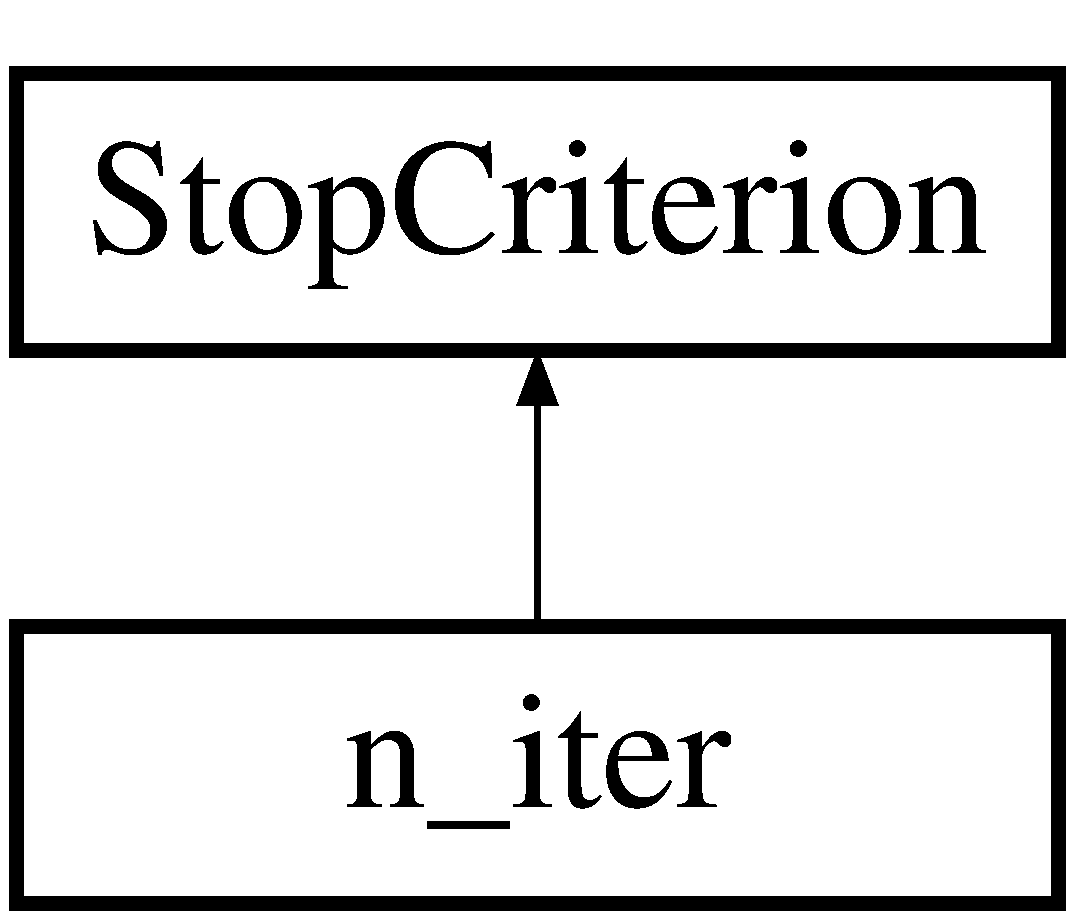
\includegraphics[height=2.000000cm]{classn__iter}
\end{center}
\end{figure}
\subsection*{Public Member Functions}
\begin{DoxyCompactItemize}
\item 
\mbox{\Hypertarget{classn__iter_a502ced9e4fb5b198b7f8d8795e610333}\label{classn__iter_a502ced9e4fb5b198b7f8d8795e610333}} 
virtual bool \mbox{\hyperlink{classn__iter_a502ced9e4fb5b198b7f8d8795e610333}{stop}} (std\+::vector$<$ double $>$ x0, std\+::vector$<$ double $>$ x1, double f0, double f1, std\+::vector$<$ double $>$ grad) override
\begin{DoxyCompactList}\small\item\em Функция, осуществляющая проверку выбранного критерия остановки и возвращающая соответсвующее значение \end{DoxyCompactList}\item 
\mbox{\Hypertarget{classn__iter_ac2024d74a52c99318dfe07fb8cf6f359}\label{classn__iter_ac2024d74a52c99318dfe07fb8cf6f359}} 
void {\bfseries Set\+\_\+n\+\_\+hat} (int n\+\_\+h)
\item 
\mbox{\Hypertarget{classn__iter_a5488180741dd37985389bc9d83760279}\label{classn__iter_a5488180741dd37985389bc9d83760279}} 
int {\bfseries Get\+\_\+n\+\_\+hat} ()
\end{DoxyCompactItemize}
\subsection*{Additional Inherited Members}


The documentation for this class was generated from the following files\+:\begin{DoxyCompactItemize}
\item 
Stop\+Criterion.\+h\item 
Stop\+Criterion.\+cpp\end{DoxyCompactItemize}

\hypertarget{classnabla}{}\section{nabla Class Reference}
\label{classnabla}\index{nabla@{nabla}}
Inheritance diagram for nabla\+:\begin{figure}[H]
\begin{center}
\leavevmode
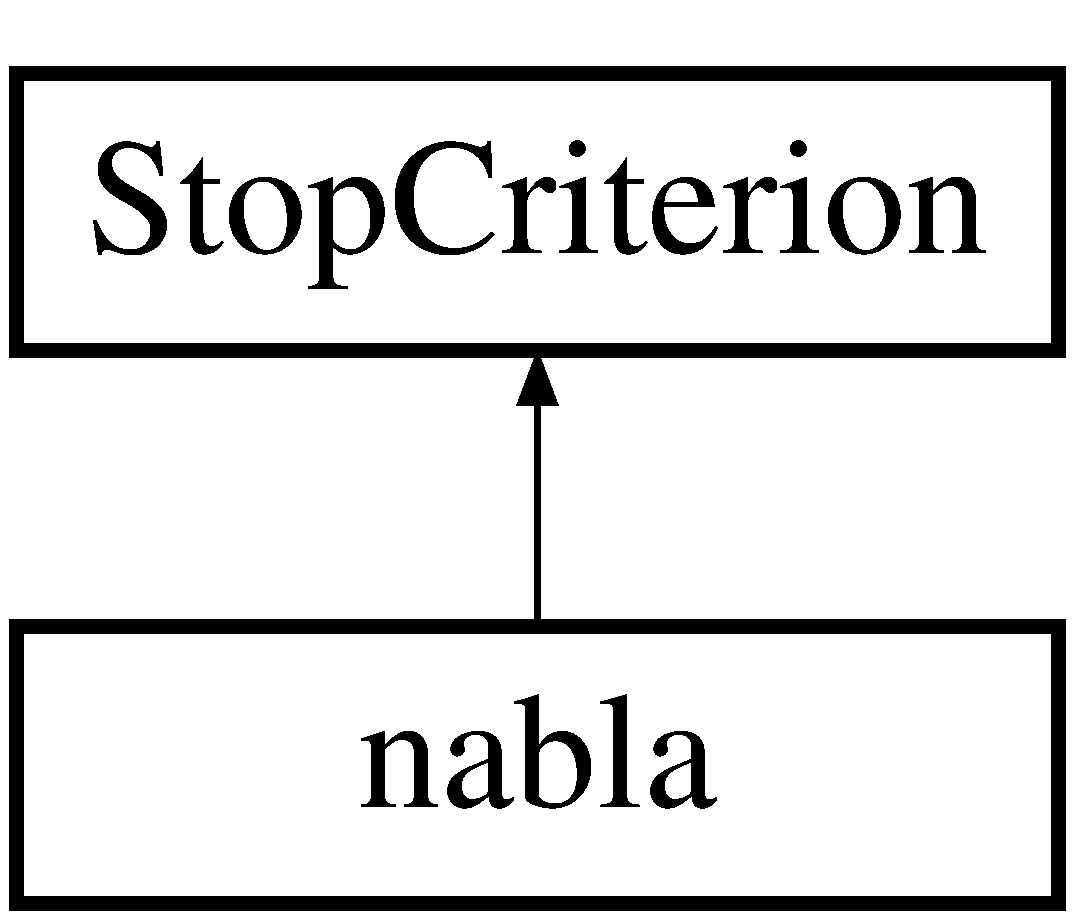
\includegraphics[height=2.000000cm]{classnabla}
\end{center}
\end{figure}
\subsection*{Public Member Functions}
\begin{DoxyCompactItemize}
\item 
\mbox{\Hypertarget{classnabla_a9c946427a24ea077555876ed4f0ecbea}\label{classnabla_a9c946427a24ea077555876ed4f0ecbea}} 
virtual bool \mbox{\hyperlink{classnabla_a9c946427a24ea077555876ed4f0ecbea}{stop}} (std\+::vector$<$ double $>$ x0, std\+::vector$<$ double $>$ x1, double f0, double f1, std\+::vector$<$ double $>$ grad) override
\begin{DoxyCompactList}\small\item\em Функция, осуществляющая проверку выбранного критерия остановки и возвращающая соответсвующее значение \end{DoxyCompactList}\end{DoxyCompactItemize}
\subsection*{Additional Inherited Members}


The documentation for this class was generated from the following files\+:\begin{DoxyCompactItemize}
\item 
Stop\+Criterion.\+h\item 
Stop\+Criterion.\+cpp\end{DoxyCompactItemize}

\hypertarget{class_optimization_method}{}\section{Optimization\+Method Class Reference}
\label{class_optimization_method}\index{Optimization\+Method@{Optimization\+Method}}


{\ttfamily \#include $<$Optimization\+Method.\+h$>$}

Inheritance diagram for Optimization\+Method\+:\begin{figure}[H]
\begin{center}
\leavevmode
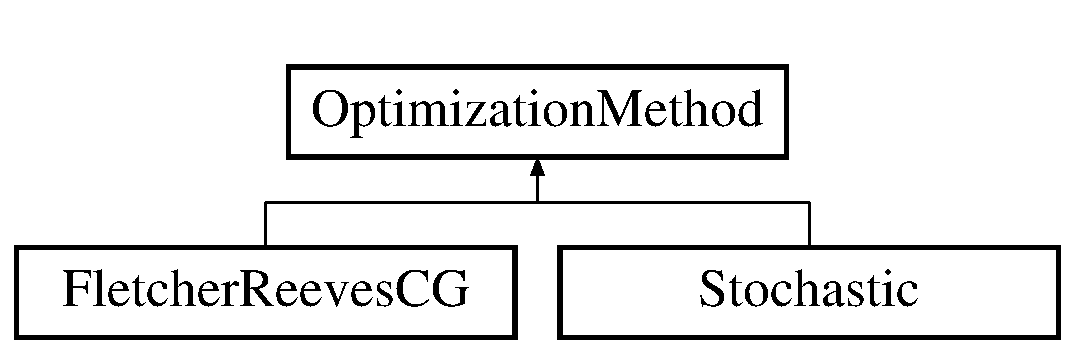
\includegraphics[height=2.000000cm]{class_optimization_method}
\end{center}
\end{figure}
\subsection*{Public Member Functions}
\begin{DoxyCompactItemize}
\item 
virtual std\+::vector$<$ double $>$ \mbox{\hyperlink{class_optimization_method_a63dd17c00593363a017c8dd440770aa2}{optimize}} (\mbox{\hyperlink{class_area}{Area}} $\ast$area, \mbox{\hyperlink{class_function}{Function}} $\ast$func, \mbox{\hyperlink{class_stop_criterion}{Stop\+Criterion}} $\ast$criterion)=0
\item 
\mbox{\Hypertarget{class_optimization_method_a8848ef8edd0cf5f7b8d28e3d91489c73}\label{class_optimization_method_a8848ef8edd0cf5f7b8d28e3d91489c73}} 
int {\bfseries Get\+\_\+iter} ()
\item 
\mbox{\Hypertarget{class_optimization_method_a4be709579f631e714fe8dc143a42e772}\label{class_optimization_method_a4be709579f631e714fe8dc143a42e772}} 
void {\bfseries Set\+\_\+x0y0y1} (std\+::vector$<$ double $>$ x)
\item 
\mbox{\Hypertarget{class_optimization_method_a50af095f319048fad7a38ea0140ec841}\label{class_optimization_method_a50af095f319048fad7a38ea0140ec841}} 
void {\bfseries Set\+\_\+eps} (double epsil)
\item 
\mbox{\Hypertarget{class_optimization_method_aa66a2635f80201526d6a17c2d0766c97}\label{class_optimization_method_aa66a2635f80201526d6a17c2d0766c97}} 
void {\bfseries Set\+\_\+limit\+\_\+iter} (int lim)
\end{DoxyCompactItemize}
\subsection*{Protected Attributes}
\begin{DoxyCompactItemize}
\item 
\mbox{\Hypertarget{class_optimization_method_acaad093b3b09087b6a4f01213b887a6e}\label{class_optimization_method_acaad093b3b09087b6a4f01213b887a6e}} 
std\+::vector$<$ double $>$ {\bfseries x0}
\item 
\mbox{\Hypertarget{class_optimization_method_a8c49149ae44f8f39e3c120221a1f3a97}\label{class_optimization_method_a8c49149ae44f8f39e3c120221a1f3a97}} 
std\+::vector$<$ double $>$ {\bfseries y0}
\item 
\mbox{\Hypertarget{class_optimization_method_a9ccddf8151dad78644c061023cde519b}\label{class_optimization_method_a9ccddf8151dad78644c061023cde519b}} 
std\+::vector$<$ double $>$ {\bfseries y1}
\item 
\mbox{\Hypertarget{class_optimization_method_aa4ae38435665f3a28b9c661e69f539b2}\label{class_optimization_method_aa4ae38435665f3a28b9c661e69f539b2}} 
int {\bfseries iter}
\item 
\mbox{\Hypertarget{class_optimization_method_af2113a4e55f9ff2f7cd65469f3fc1a55}\label{class_optimization_method_af2113a4e55f9ff2f7cd65469f3fc1a55}} 
double {\bfseries eps}
\item 
\mbox{\Hypertarget{class_optimization_method_a724a0ba7ab2a661bc495680fc15006e0}\label{class_optimization_method_a724a0ba7ab2a661bc495680fc15006e0}} 
int {\bfseries limit\+\_\+iter}
\end{DoxyCompactItemize}


\subsection{Detailed Description}
Данный класс содержит два метода оптимизации нахождения минимума заданной функции в заданной области\+:
\begin{DoxyItemize}
\item Итерационный (здесь метод сопряженных градиентов Флетчера-\/Ривса)
\item Стохастический 
\end{DoxyItemize}

\subsection{Member Function Documentation}
\mbox{\Hypertarget{class_optimization_method_a63dd17c00593363a017c8dd440770aa2}\label{class_optimization_method_a63dd17c00593363a017c8dd440770aa2}} 
\index{Optimization\+Method@{Optimization\+Method}!optimize@{optimize}}
\index{optimize@{optimize}!Optimization\+Method@{Optimization\+Method}}
\subsubsection{\texorpdfstring{optimize()}{optimize()}}
{\footnotesize\ttfamily virtual std\+::vector$<$double$>$ Optimization\+Method\+::optimize (\begin{DoxyParamCaption}\item[{\mbox{\hyperlink{class_area}{Area}} $\ast$}]{area,  }\item[{\mbox{\hyperlink{class_function}{Function}} $\ast$}]{func,  }\item[{\mbox{\hyperlink{class_stop_criterion}{Stop\+Criterion}} $\ast$}]{criterion }\end{DoxyParamCaption})\hspace{0.3cm}{\ttfamily [pure virtual]}}

Функция нахождения минимума функции и точки, в которой он достигается 
\begin{DoxyParams}{Parameters}
{\em area} & Выбранная область, в которой будет находиться минимум \\
\hline
{\em func} & Функция, минимум которой будет находиться \\
\hline
{\em criterion} & Критерий остановки для выбранного метода \\
\hline
\end{DoxyParams}
\begin{DoxyReturn}{Returns}
Точку минимума функции в области 
\end{DoxyReturn}


Implemented in \mbox{\hyperlink{class_stochastic_a7a219f4e02daecd5c8c185de0df80353}{Stochastic}}, and \mbox{\hyperlink{class_fletcher_reeves_c_g_a40c56c0485371b31000672236b433dc7}{Fletcher\+Reeves\+CG}}.



The documentation for this class was generated from the following files\+:\begin{DoxyCompactItemize}
\item 
Optimization\+Method.\+h\item 
Optimization\+Method.\+cpp\end{DoxyCompactItemize}

\hypertarget{class_rect_area}{}\section{Rect\+Area Class Reference}
\label{class_rect_area}\index{Rect\+Area@{Rect\+Area}}
Inheritance diagram for Rect\+Area\+:\begin{figure}[H]
\begin{center}
\leavevmode
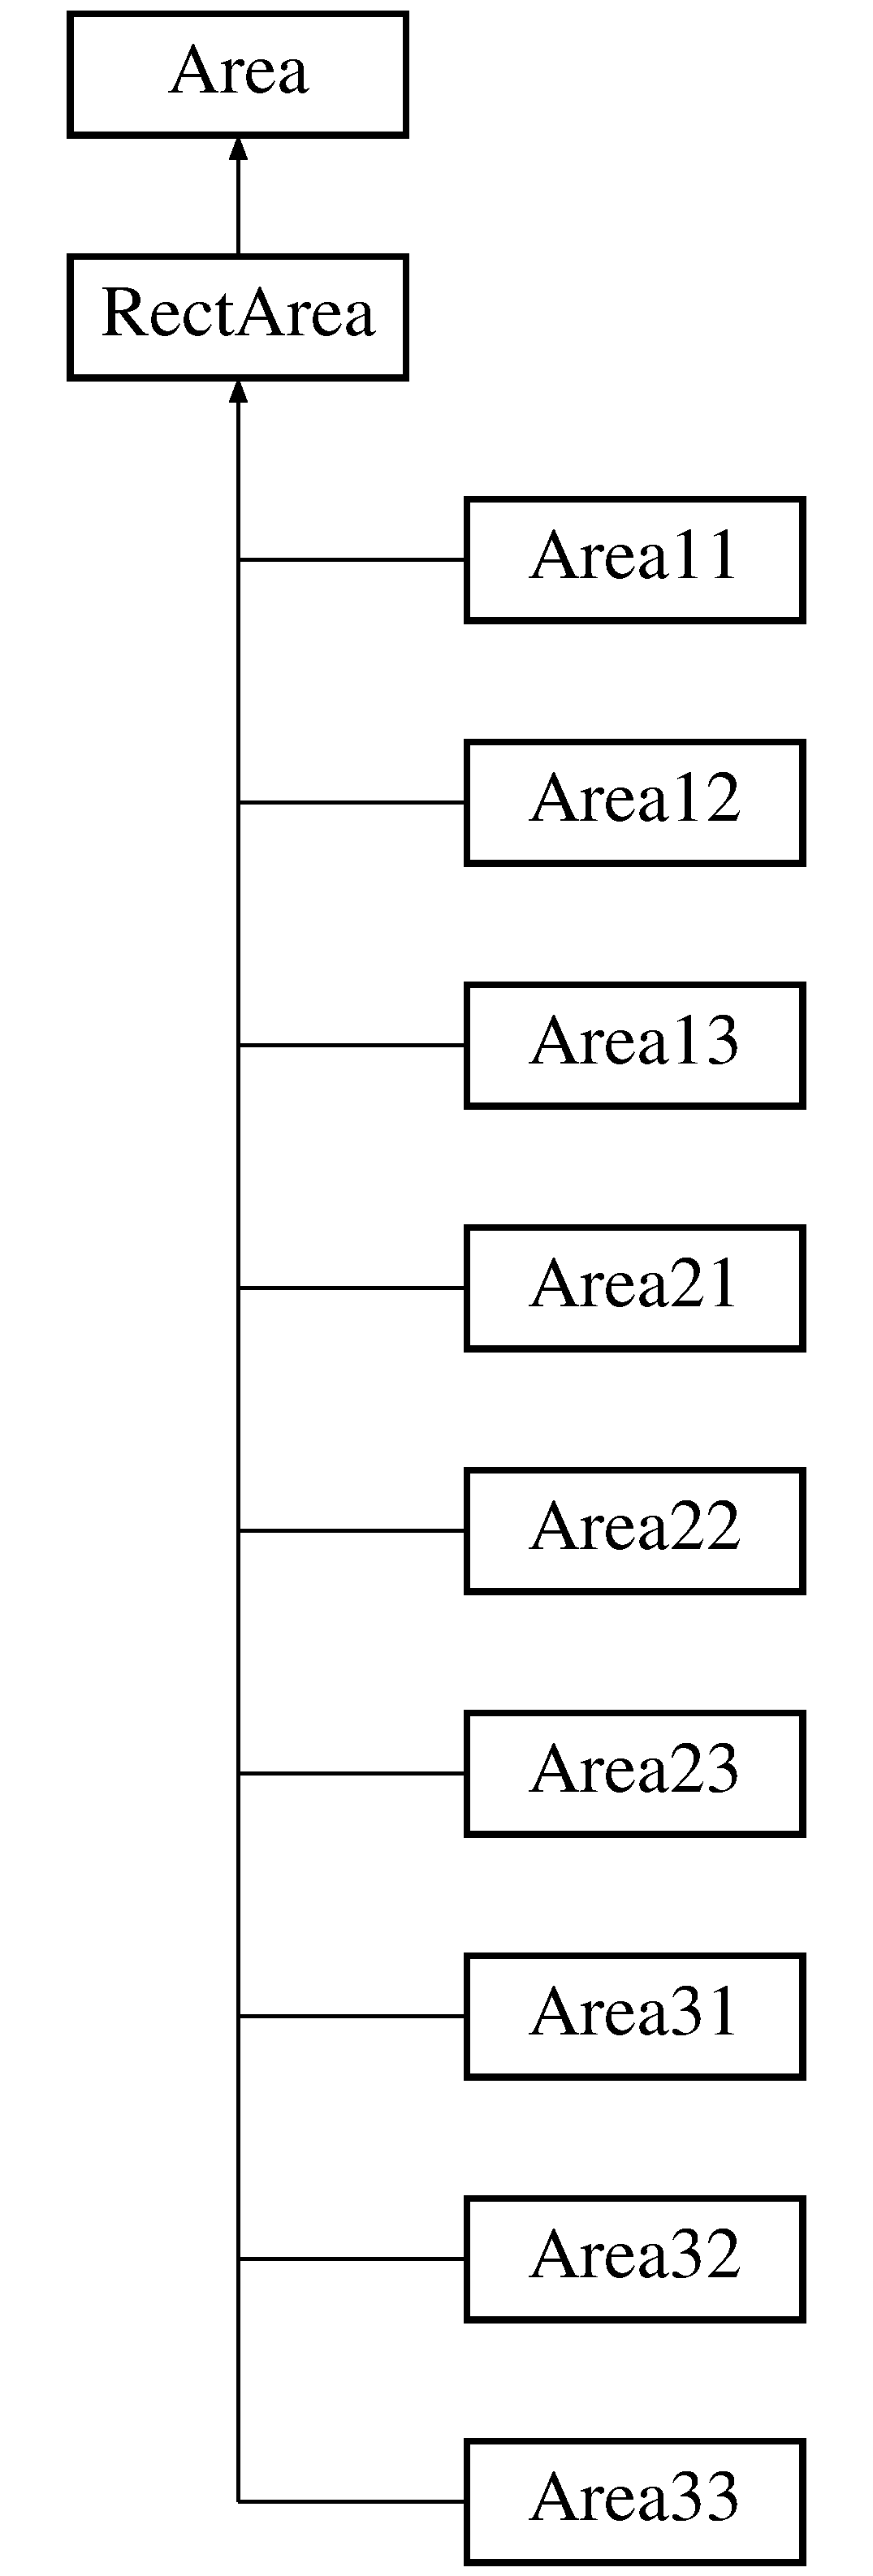
\includegraphics[height=11.000000cm]{class_rect_area}
\end{center}
\end{figure}
\subsection*{Public Member Functions}
\begin{DoxyCompactItemize}
\item 
\mbox{\Hypertarget{class_rect_area_adf9ff960f6184aa6dabec01e78a0d4d4}\label{class_rect_area_adf9ff960f6184aa6dabec01e78a0d4d4}} 
{\bfseries Rect\+Area} (int n, std\+::vector$<$ double $>$ dot)
\end{DoxyCompactItemize}
\subsection*{Additional Inherited Members}


The documentation for this class was generated from the following file\+:\begin{DoxyCompactItemize}
\item 
Area.\+h\end{DoxyCompactItemize}

\hypertarget{class_stochastic}{}\section{Stochastic Class Reference}
\label{class_stochastic}\index{Stochastic@{Stochastic}}
Inheritance diagram for Stochastic\+:\begin{figure}[H]
\begin{center}
\leavevmode
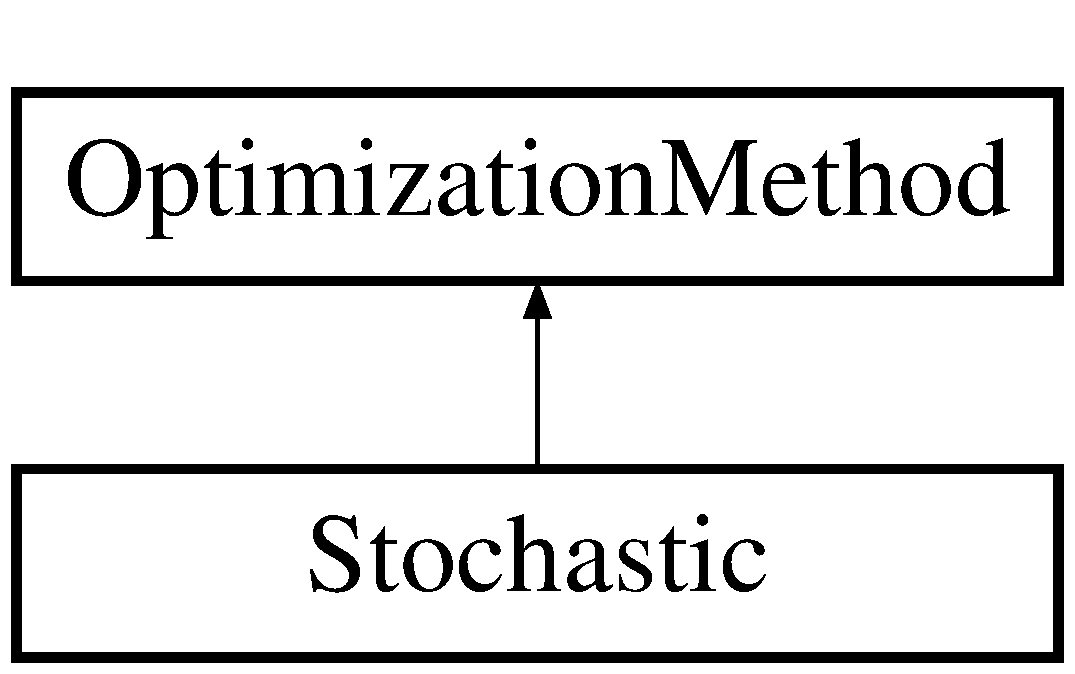
\includegraphics[height=2.000000cm]{class_stochastic}
\end{center}
\end{figure}
\subsection*{Public Member Functions}
\begin{DoxyCompactItemize}
\item 
virtual std\+::vector$<$ double $>$ \mbox{\hyperlink{class_stochastic_a7a219f4e02daecd5c8c185de0df80353}{optimize}} (\mbox{\hyperlink{class_area}{Area}} $\ast$area, \mbox{\hyperlink{class_function}{Function}} $\ast$func, \mbox{\hyperlink{class_stop_criterion}{Stop\+Criterion}} $\ast$criterion) override
\item 
\mbox{\Hypertarget{class_stochastic_ad66c12f98a754caea907d5df26af56ef}\label{class_stochastic_ad66c12f98a754caea907d5df26af56ef}} 
void {\bfseries Set\+\_\+prob} (double p)
\end{DoxyCompactItemize}
\subsection*{Additional Inherited Members}


\subsection{Member Function Documentation}
\mbox{\Hypertarget{class_stochastic_a7a219f4e02daecd5c8c185de0df80353}\label{class_stochastic_a7a219f4e02daecd5c8c185de0df80353}} 
\index{Stochastic@{Stochastic}!optimize@{optimize}}
\index{optimize@{optimize}!Stochastic@{Stochastic}}
\subsubsection{\texorpdfstring{optimize()}{optimize()}}
{\footnotesize\ttfamily std\+::vector$<$ double $>$ Stochastic\+::optimize (\begin{DoxyParamCaption}\item[{\mbox{\hyperlink{class_area}{Area}} $\ast$}]{area,  }\item[{\mbox{\hyperlink{class_function}{Function}} $\ast$}]{func,  }\item[{\mbox{\hyperlink{class_stop_criterion}{Stop\+Criterion}} $\ast$}]{criterion }\end{DoxyParamCaption})\hspace{0.3cm}{\ttfamily [override]}, {\ttfamily [virtual]}}

Функция нахождения минимума функции и точки, в которой он достигается 
\begin{DoxyParams}{Parameters}
{\em area} & Выбранная область, в которой будет находиться минимум \\
\hline
{\em func} & Функция, минимум которой будет находиться \\
\hline
{\em criterion} & Критерий остановки для выбранного метода \\
\hline
\end{DoxyParams}
\begin{DoxyReturn}{Returns}
Точку минимума функции в области 
\end{DoxyReturn}


Implements \mbox{\hyperlink{class_optimization_method_a63dd17c00593363a017c8dd440770aa2}{Optimization\+Method}}.



The documentation for this class was generated from the following files\+:\begin{DoxyCompactItemize}
\item 
Optimization\+Method.\+h\item 
Optimization\+Method.\+cpp\end{DoxyCompactItemize}

\hypertarget{class_stop_criterion}{}\section{Stop\+Criterion Class Reference}
\label{class_stop_criterion}\index{Stop\+Criterion@{Stop\+Criterion}}


{\ttfamily \#include $<$Stop\+Criterion.\+h$>$}

Inheritance diagram for Stop\+Criterion\+:\begin{figure}[H]
\begin{center}
\leavevmode
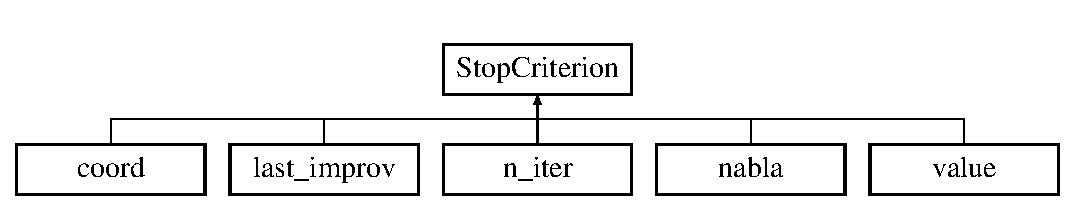
\includegraphics[height=2.000000cm]{class_stop_criterion}
\end{center}
\end{figure}
\subsection*{Public Member Functions}
\begin{DoxyCompactItemize}
\item 
\mbox{\Hypertarget{class_stop_criterion_a5d6cb226bf9fc09d2924941f382f945a}\label{class_stop_criterion_a5d6cb226bf9fc09d2924941f382f945a}} 
virtual bool \mbox{\hyperlink{class_stop_criterion_a5d6cb226bf9fc09d2924941f382f945a}{stop}} (std\+::vector$<$ double $>$ x0, std\+::vector$<$ double $>$ x1, double f0, double f1, std\+::vector$<$ double $>$ grad)=0
\begin{DoxyCompactList}\small\item\em Функция, осуществляющая проверку выбранного критерия остановки и возвращающая соответсвующее значение \end{DoxyCompactList}\item 
\mbox{\Hypertarget{class_stop_criterion_abbd042a803864e4da709b29f5c34ef2d}\label{class_stop_criterion_abbd042a803864e4da709b29f5c34ef2d}} 
void {\bfseries Set\+\_\+eps} (double epsil)
\end{DoxyCompactItemize}
\subsection*{Protected Attributes}
\begin{DoxyCompactItemize}
\item 
\mbox{\Hypertarget{class_stop_criterion_aa848cdc8c317a0788f3bc2daa9444b18}\label{class_stop_criterion_aa848cdc8c317a0788f3bc2daa9444b18}} 
double {\bfseries eps}
\item 
\mbox{\Hypertarget{class_stop_criterion_ad42a03c72fd52d679c1bd787761cb73a}\label{class_stop_criterion_ad42a03c72fd52d679c1bd787761cb73a}} 
double {\bfseries eps\+\_\+2}
\end{DoxyCompactItemize}


\subsection{Detailed Description}
Данный класс содержит определения различных критериев остановки для разных методов\+:
\begin{DoxyItemize}
\item Итерационный метод\+:
\begin{DoxyItemize}
\item Норма градиента меньше эпсилон
\item Норма разности двух соседних точек меньше эпсилон
\item Модуль разности значений в двух соседних точках, деленной на значение в последней меньше эпсилон
\end{DoxyItemize}
\item Стохастический метод\+:
\begin{DoxyItemize}
\item Превышение числа итераций с последнего улучшения
\item Модуль разности значений с последнего улучшения 
\end{DoxyItemize}
\end{DoxyItemize}

The documentation for this class was generated from the following files\+:\begin{DoxyCompactItemize}
\item 
Stop\+Criterion.\+h\item 
Stop\+Criterion.\+cpp\end{DoxyCompactItemize}

\hypertarget{classvalue}{}\section{value Class Reference}
\label{classvalue}\index{value@{value}}
Inheritance diagram for value\+:\begin{figure}[H]
\begin{center}
\leavevmode
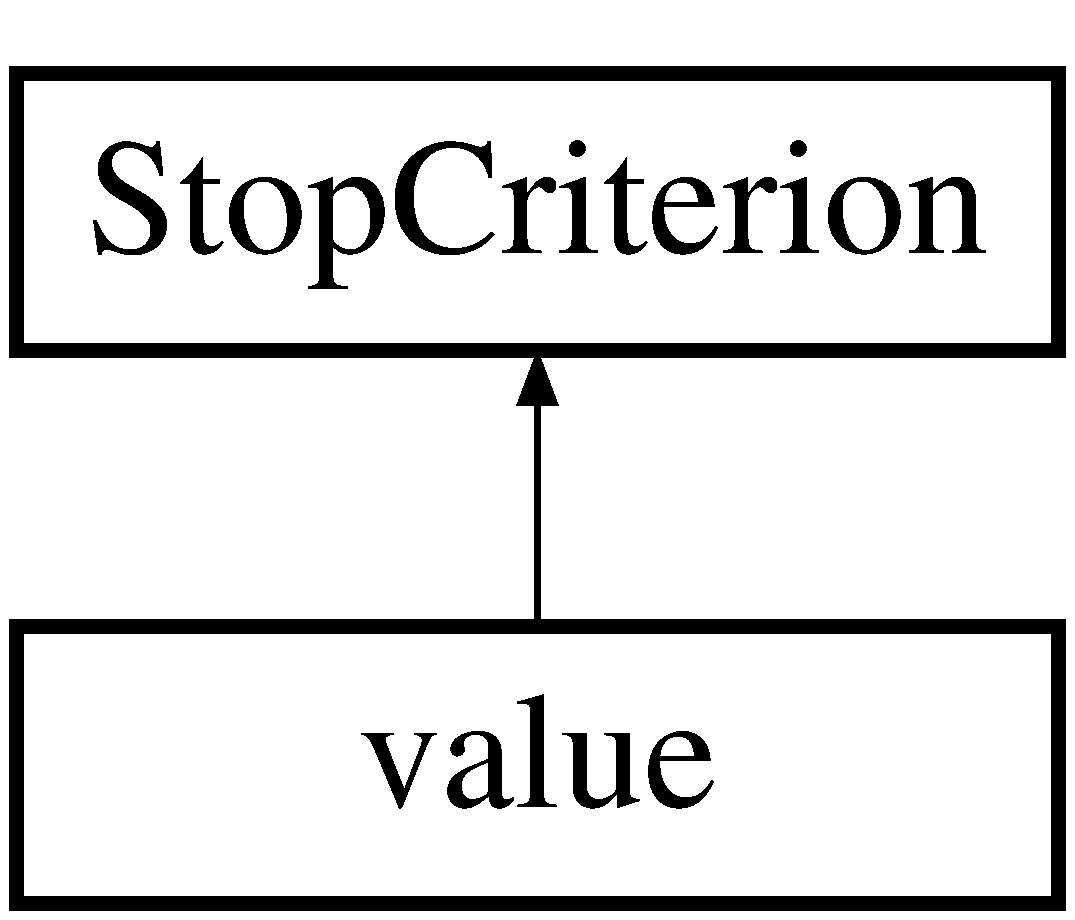
\includegraphics[height=2.000000cm]{classvalue}
\end{center}
\end{figure}
\subsection*{Public Member Functions}
\begin{DoxyCompactItemize}
\item 
\mbox{\Hypertarget{classvalue_a025d523b94d9124d42b7622ebfd7a09e}\label{classvalue_a025d523b94d9124d42b7622ebfd7a09e}} 
virtual bool \mbox{\hyperlink{classvalue_a025d523b94d9124d42b7622ebfd7a09e}{stop}} (std\+::vector$<$ double $>$ x0, std\+::vector$<$ double $>$ x1, double f0, double f1, std\+::vector$<$ double $>$ grad) override
\begin{DoxyCompactList}\small\item\em Функция, осуществляющая проверку выбранного критерия остановки и возвращающая соответсвующее значение \end{DoxyCompactList}\end{DoxyCompactItemize}
\subsection*{Additional Inherited Members}


The documentation for this class was generated from the following files\+:\begin{DoxyCompactItemize}
\item 
Stop\+Criterion.\+h\item 
Stop\+Criterion.\+cpp\end{DoxyCompactItemize}

%--- End generated contents ---

% Index
\backmatter
\newpage
\phantomsection
\clearemptydoublepage
\addcontentsline{toc}{chapter}{Index}
\printindex

\end{document}
